%\chapter{Derivation of an illumination model for sea surfaces}
\chapter{An illumination model for sea surfaces}
\label{apdx:illumination_model_derivation}

In this appendix, an analytical model of the optical properties of water surfaces is derived. If a part of the \idxs{wave}{spectrum} is discarded, such as the part containing all frequencies that are too large to be properly visualized or properly represented on the simulation grid, details on the water surface will be lost which --- for \visualization purposes --- need compensation in the form of increased \idxse{diffuse}{reflection}{diffuseness} in the \reflections on the water surface.

The model derived here will compensate for this loss of detail, and is based on the statistical distribution of the gradient of the free surface elevation. What started out as a simple idea was written down on paper and tried out, and soon resulted in a long chain of equations --- a work that was done outside of the scope of this thesis work. Furthermore, as it turned out, similar analytical models had already been developed earlier, for example by \citet{Caillault2007}. Anyway, what follows in this appendix is the derivation of a new model.

\section{Microfacets}

If we assume that some of the frequencies have been removed from the rendering, it becomes impossible to treat those frequencies directly. However, it is still possible to treat them statistically.

To model the water surface, we will use something known as \microfacets. These are basically are infinitesimal surface elements, tiled one after another, and are on a much smaller \scale than what is represented in the \rendering. The \idxs{surface}{normal} of these microfacets is \assumed to be \stochastically distributed with a known \idxs{probability}{distribution} --- we will cover this later.

The idea is that if we know the \idxs{probability}{distribution} for all removed frequencies, we can calculate the distribution for the surface normal. This makes it possible to calculate the distribution for the \idxs{reflection}{direction} of a \ray that is \reflected on the water surface, for a certain \idxs{incident}{direction}. This in turn makes it possible to calculate the likelihood that the object of which the reflection that can be seen in a specific point on the surface is --- for example --- the \sun.

This means that we can calculate the average brightness of a point on the surface as perceived by the observer. Besides, if we \assume that the removed frequencies correspond to waves that are so short that the crests become indistinguishable from one another (this is more likely if the observer has bad sight), the average brightness will probably also be a good approximation of the actual brightness perceived by the observer. But before we can start to calculate the average brightness, we need to make a few \assumptions.

First, let's \assume that all frequencies of the wave spectrum are \superposed linearly on top of each other. This implies that there is no \idxs{horizontal}{displacement} --- that is, either the waves are not \idxsp{Gerstner}{wave}{s}, or the \idxs{wave}{amplitude} is so much smaller than the \wavelength that we can neglect whether the waves are Gerstner waves or not.

Second, to make things simpler, let's \assume that both the fraction of the water surface that is masked behind other waves, and hence is not visible to the observer, and the fraction of the surface that is \shadowed by other waves, are so close to zero they can be neglected. In other words, our \microfacets can be assumed to not hide any of the other microfacets, either from the sun or from the observer.

Third, let's also assume that no light will ever be reflected twice on the water surface before reaching the observer.

Now, let's denote the \index{elevation!free surface|see{free surface elevation}}\idxs{free}{surface elevation} of the actual water surface as $\eta^*$, and the free surface elevation of the simplified surface (from which a part of the wave spectrum has been discarded) as $\eta$, and let these be functions of $\vec{r}$, which is a \twodimensional vector in the horizontal plane. We can start by noting that $\eta$ is less detailed than $\eta^*$, and that it doesn't contain all information about the actual water surface, whereas $\eta^*$ does. Furthermore, while $\eta$ is known, $\eta^*$ is not.

We can therefore only calculate the normal of the simplified surface --- let's call this normal $\normvec{n}$. Let's also define the \idx{anti-normalization} $\anormvec{\xi}$ of a vector $\vec{\xi}$ as
%
\begin{equation} \label{eq:anti_normal_definition}
\anormvec{\xi} \,=\, \frac{\vec{\xi}}{\normvec{z}\cdot\vec{\xi}}\,,
\end{equation}
%
where $\normvec{z}$ is the \idxs{unit}{vector} in the positive vertical direction (which is the negation of the direction of the \idxs{gravitational acceleration}{vector}, or the normal of a flat water surface). This implies that the $\normvec{z}$-component of an anti-normalized vector always is 1. Note that the anti-normalization of a vector is only defined if the original vector has a non-zero $\normvec{z}$-component, and that it --- when defined --- is parallel to the original vector. The \idx{anti-normal} $\anormvec{n}$ of the surface $\eta$ becomes
%
\begin{equation} \label{eq:anti_normal_from_gradient}
\anormvec{n} \,=\, \left(\!\!\!\begin{array}{c}-\nabla\eta(\vec{r}\,) \\ 1\end{array}\!\!\!\right),
\end{equation}
%
where the last component is the $\normvec{z}$-component. The \gradient in turn can be written as
%
\begin{equation}
\nabla\eta(\vec{r}\,) \,=\, \nabla\mathcal{F}^{-1}\{\fdfunc{\eta}(\vec{k}\,)\}(\vec{r}\,) \,=\, \mathcal{F}^{-1}\{\vec{k}\,\fdfunc{\eta}(\vec{k}\,)\}(\vec{r}\,),
\end{equation}
%
where $\mathcal{F}^{-1}$ is the \index{operator!inverse non-unitary Fourier transform|see{inverse non-unitary Fourier transform operator}}\index{non-unitary Fourier transform operator!inverse|see{inverse non-unitary Fourier transform operator}}\idxs{inverse non-unitary}{Fourier transform operator}, $\fdfunc{\eta}(\vec{k}\,)$ is the \idxs{Fourier}{transform} of $\eta(\vec{r}\,)$ and $\vec{k}$ is the \idxs{wave}{vector}. Since $\eta^*$ is unknown, the anti-normal of the real surface, $\anormvec{n}^*$, cannot be calculated, although it can still be written as
%
\begin{equation} \label{eq:eta_anti_normal}
\anormvec{n}^* \,=\, \left(\!\!\!\begin{array}{c}-\nabla\eta^*(\vec{r}\,) \\ 1\end{array}\!\!\!\right),
\end{equation}
%
where the gradient in turn can be written as
%
\begin{equation}
\nabla\eta^*(\vec{r}\,) \,=\, \mathcal{F}^{-1}\{\vec{k}\,\fdfunc{\eta}^*(\vec{k}\,)\}(\vec{r}\,),
\end{equation}
%
where $\fdfunc{\eta}^*(\vec{k}\,)$ is the \idxs{Fourier}{transform} of $\eta^*$. However, only the part of $\fdfunc{\eta}^*(\vec{k}\,)$ where the wave spectrum has not been cut off is known; in fact, this part is equal to $\fdfunc{\eta}(\vec{k}\,)$, while the reminding part of $\fdfunc{\eta}^*(\vec{k}\,)$ is unknown. On the other hand, if we know what the \idxs{wave}{spectrum} looks like, we can calculate the \idxs{probability}{distribution} of $\eta^*$.

If $\vec{r}$ is assumed to be \idxse{uniform}{distribution}{uniformly distributed} over a large surface area, i.e. there is no \bias in the distribution of $\vec{r}$ regarding to the surface slope $\nabla\eta^*$, or any other local property of the surface for that matter, the distribution of $\fdfunc{\eta}^*$ is easily obtained by looking at the wave spectrum. And from that distribution we will be able to get something that is more valuable to us, namely the distribution of $\nabla\eta^*$.

\subsection{Wave spectra}

When using a \idxs{wave}{spectrum}, the free surface elevation is considered indeterministic, that is, \stochastic. Let's consider $\psi$ to be a completely unknown free surface elevation (as opposed to $\eta^*$, for which the \idxs{frequency}{domain} representation $\fdfunc{\eta}^*$ known in a part of the spectrum but unknown everywhere else). Almost every \idxs{wave}{spectrum}, $S$, used in \idxs{computer}{graphics}, is a function of the wave vector $\vec{k}$ and gives the \variance of the free surface elevation per unit \idxs{reciprocal}{length} squared (the elements of $\vec{k}$ are reciprocal lengths), and thus has the unit $\text{m}^4$. 

If $S$ assumes that the wave components corresponding to the wave vectors are on the exponential form $e^{i(\vec{k}\cdot\vec{r}-\omega t)}$, which is what $\fdfunc{\psi}$ also assumes, rather than on the \sinusoidal form $\sin(\vec{k}\cdot\vec{r}-\omega t)$, which otherwise is a pretty common case in computer graphics, this means that
%
\begin{equation} \label{eq:wave_spectrum_definition}
S(\vec{k}\,) \,=\, \frac{\opd \Var(\psi)}{\opd\vec{k}},
\end{equation}
%
where $\Var$ is the \idxs{variance}{operator} with respect to $\vec{r}$ ($\vec{r}$ is considered to be stochastically distributed), for a fixed time $t$, and $\opd\vec{k}$ is an \infinitesimal \idxs{reciprocal}{area} element, centered around $\vec{k}$. Here, $\opd\Var(\psi)$ denotes the additional variance within $\psi$ caused solely by the part of the wave spectrum specified by $\opd\vec{k}$.

\eqref{eq:wave_spectrum_definition} implies that the additional variance in $\psi$ --- $\Var_{\Delta\vec{k}}(\psi)$ --- caused by a part of the wave spectrum specified by a reciprocal area element $\Delta\vec{k}$ is
%
\begin{equation} \label{eq:variance_k_eta}
\Var_{\Delta\vec{k}}(\psi) \,=\, \int_{\Delta\vec{k}}\opd \Var(\psi) \,=\, \int_{\Delta\vec{k}}\frac{\opd \Var(\psi)}{\opd\vec{k}}\opd\vec{k} \,=\, \int_{\Delta\vec{k}}S(\vec{k}\,)\opd\vec{k}.
\end{equation}

Since the variance doesn't \correlate wave components of different \wavelengths, we have
%
\begin{equation} \label{eq:variance_k_eta_to_variance_eta_k}
\Var(\psi_{\Delta\vec{k}}) \,=\, \Var_{\Delta\vec{k}}(\psi),
\end{equation}
%
where $\psi_{\Delta\vec{k}}$ is defined as
%
\begin{equation} \label{eq:eta_k_of_fd_eta_k}
\psi_{\Delta\vec{k}} \,=\, \mathcal{F}^{-1}\{\fdfunc{\psi}_{\Delta\vec{k}}(\vec{k}\,)\},
\end{equation}
%
where in turn
%
\begin{equation} \label{eq:fd_eta_delta_k_definition}
\fdfunc{\psi}_{\Delta\vec{k}}(\vec{k}\,) \,=\, \begin{cases}
\fdfunc{\psi}(\vec{k}\,), & \vec{k} \in \Delta\vec{k} \\
0, & \text{otherwise}
\end{cases}.
\end{equation}

Here, $\fdfunc{\psi}$ is the \idxs{non-unitary}{Fourier transform} of $\psi$, i.e.\ $\fdfunc{\psi}(\vec{k}\,) = \mathcal{F}\{\psi(\vec{r}\,)\}(\vec{k}\,)$. Besides, the time average of $\fdfunc{\psi}(\vec{k}\,)$ is assumed to be 0 for any given wave vector $\vec{k}$, that is
%
\begin{equation} \label{eq:zero_expectation_value_reciprocal_space}
\E_{\vec{k}}[\fdfunc{\psi}] \,=\, 0,\ \forall\ \vec{k},
\end{equation}
%
where $\E_{\vec{k}}$ is the \idxs{expectation value}{operator} with respect to time, for a fixed value of $\vec{k}$, and can be defined as
%
\begin{equation} \label{eq:expectation_value_reciprocal_space_with_regard_to_t_definition}
\E_{\vec{k}}[\fdfunc{f}] \,=\, \lim_{T\to\infty}\frac{1}{T}\int_0^T \fdfunc{f}(\vec{k},\,t)\opd t,
\end{equation}
%
where $\fdfunc{f}$ is an arbitrary function of $\vec{k}$ and $t$. After \idxsp{inverse}{Fourier transform}{ing} \eqref{eq:zero_expectation_value_reciprocal_space}, this also results in 
%
\begin{equation} \label{eq:zero_expectation_value_real_space_with_regard_to_t}
\E_{\vec{r}}[\psi] \,=\, 0,\ \forall\ \vec{r},
\end{equation}
%
where $\E_{\vec{r}}$ is the \idxs{expectation value}{operator} with respect to time, for a fixed value of $\vec{r}$, and can be defined as
%
\begin{equation} \label{eq:expectation_value_real_space_with_regard_to_t_definition}
\E_{\vec{r}}[f] \,=\, \lim_{T\to\infty}\frac{1}{T}\int_0^T f(\vec{r},\,t)\opd t,
\end{equation}
%
where $f$ is an arbitrary function of $\vec{r}$ and $t$.

Let's assume that $\psi$ is periodic in both of the horizontal dimensions with the period $P$ (this is a common trick in \idxs{computer}{graphics}) with a large, square surface element $A$ (with \mbox{$|A| = P^2$}) that keeps repeating itself, such that
%
\begin{equation} \label{eq:water_surface_periodicity}
\psi(\vec{r}+P\normvec{x}) \,=\, \psi(\vec{r}+P\normvec{y}) \,=\, \psi(\vec{r}\,),\ \forall\ \vec{r},
\end{equation}
%
where $\normvec{x}$ and $\normvec{y}$ are the \index{vector!orthonormal basis|see{orthonormal basis vector}}\idxsp{orthonormal}{basis vector}{s} generating the \idxs{horizontal}{plane}. This implies that $\fdfunc{\psi}$ is discrete, with \idxsp{Dirac}{impulse}{s} arranged in the intersection points of a square grid with the size $d = 2\pi/P$, such that
%
\begin{equation} \label{eq:fd_eta_series}
\renewcommand*{\arraystretch}{2}
\begin{array}{c}
\displaystyle \fdfunc{\psi}(\vec{k}\,) \,=\, 4\pi^2\sum_{m=-\infty}^{+\infty}\sum_{n=-\infty}^{+\infty} \fdfunc{\psi}(m,\,n)\,\delta(\vec{k} - md\normvec{x} - nd\normvec{y}) \\
\displaystyle =\, 4\pi^2\sum_{m=-\infty}^{+\infty}\sum_{n=-\infty}^{+\infty} \fdfunc{\psi}(m,\,n)\,\delta(\vec{k} - \vec{k}_{m,n}),
\end{array}
\end{equation}
%
where $\fdfunc{\psi}(m,\,n)$ is a \twodimensional \sequence of coefficients associated with $\fdfunc{\psi}$, $m$ and $n$ are two integers used to index the terms in the \series, and $\vec{k}_{m,n} = md\normvec{x} + nd\normvec{y}$.

\comment
{
By \assuming that $\vec{r}$ is \idxse{uniform}{distribution}{uniformly distributed} within $A$, the \idxs{variance}{operator} with respect to $\vec{r}$ can be defined as

\begin{equation} \label{eq:variance_periodic_function_definition}
\Var(f) \,=\, \E_{A,t}[\,|f - \E_{A,t}[f]\,|^2\,],
\end{equation}

where $\E_{A,t}$ denotes the \idxs{expectation value}{operator} with regard to  $\vec{r}$ (which is uniformly distributed within $A$), for a fixed time $t$, and can be defined as

\begin{equation} \label{eq:expectation_value_with_regard_to_r_definition}
\E_{A,t}[f] \,=\, \frac{1}{|A|}\int_A f(\vec{r},\,t)\opd\vec{r}.
\end{equation}

By realizing that this \idxs{expectation}{value} will be time independent for $f(\vec{r}\,) = \varphi(\vec{r}\,)$, where $\varphi$ is any periodic (obeying \eqref{eq:water_surface_periodicity}), free surface elevation that conserves mass, meaning that the integral over $A$ is time independent, we can use \eqref{eq:zero_expectation_value_real_space_with_regard_to_t} and \eqref{eq:expectation_value_with_regard_to_t_definition} to get

\begin{equation} \label{eq:zero_expectation_value_real_space_with_regard_to_r}
\renewcommand*{\arraystretch}{2}
\begin{array}{c}
\displaystyle \E_{A,t}[\varphi] \,=\, \frac{1}{|A|}\int_A \varphi(\vec{r},\,t)\opd\vec{r} \,=\, \lim_{T\to\infty}\frac{1}{T}\int_0^T\frac{1}{|A|}\int_A \varphi(\vec{r},\,t)\opd\vec{r}\opd t \\
\displaystyle =\, \frac{1}{|A|}\int_A\lim_{T\to\infty}\frac{1}{T}\int_0^T \varphi(\vec{r},\,t)\opd t\opd\vec{r} \,=\, \frac{1}{|A|}\int_A \E_{\vec{r}}[\varphi]\opd\vec{r} \,=\, 0.
\end{array}
\end{equation}

By using using \eqref{eq:expectation_value_with_regard_to_r_definition} and \eqref{eq:zero_expectation_value_real_space_with_regard_to_r}, \eqref{eq:variance_periodic_function_definition} becomes

\begin{equation} \label{eq:variance_integral}
\Var(\varphi) \,=\, \frac{1}{|A|}\int_A|\varphi(\vec{r}\,)|^2\opd\vec{r}.
\end{equation}
}

\eqref{eq:fd_eta_series} can be reduced to
%
\begin{equation} \label{eq:fd_eta_series_reduced}
\fdfunc{\psi}(\vec{k}\,) \,=\, \sum_{m=-\infty}^{+\infty}\sum_{n=-\infty}^{+\infty} \fdfunc{\psi}_{m,n}(\vec{k}\,),
\end{equation}
%
where
%
\begin{equation} \label{eq:fd_eta_mn_definition}
\fdfunc{\psi}_{m,n}(\vec{k}\,) \,=\, 4\pi^2 \fdfunc{\psi}(m,\,n)\,\delta(\vec{k} - \vec{k}_{m,n}),
\end{equation}
%
and if we define $\Delta\vec{k}_{m,n}$ as a square that has the side $d$, is aligned with $\normvec{x}$ and $\normvec{y}$ and is centered in $\vec{k}_{m,n}$, we see that
%
\begin{equation} \label{eq:fd_eta_dk_mn_definition}
\fdfunc{\psi}_{\Delta\vec{k}_{m,n}}(\vec{k}\,) \,=\, \fdfunc{\psi}_{m,n}(\vec{k}\,).
\end{equation}
%
It follows naturally to do the same thing with the real space representation, $\psi(\vec{r}\,)$, and write that as
%
\begin{equation} \label{eq:eta_series_reduced}
\psi(\vec{r}\,) \,=\, \sum_{m=-\infty}^{+\infty}\sum_{n=-\infty}^{+\infty} \psi_{m,n}(\vec{r}\,),
\end{equation}
%
where
%
\begin{equation} \label{eq:eta_mn_definition}
\renewcommand*{\arraystretch}{1.5}
\begin{array}{c}
\displaystyle \psi_{m,n}(\vec{r}\,) \,=\, \mathcal{F}^{-1}\{\fdfunc{\psi}_{m,n}(\vec{k}\,)\}(\vec{r}\,) \,=\, \frac{1}{(2\pi)^2} \int_{\mathbb{R}^2} \fdfunc{\psi}_{m,n}(\vec{k}\,) e^{i\vec{k}\cdot\vec{r}}\opd \vec{k} \\
\displaystyle =\, \frac{1}{4\pi^2} \int_{\mathbb{R}^2} 4\pi^2\,\fdfunc{\psi}(m,\,n)\,\delta(\vec{k} - md\normvec{x} - nd\normvec{y}) e^{i\vec{k}\cdot\vec{r}}\opd \vec{k} \,=\, \fdfunc{\psi}(m,\,n)\,e^{i\vec{k}_{m,n}\cdot\vec{r}}.
\end{array}
\end{equation}
%
Taking the gradient of this yields
%
\begin{equation} \label{eq:grad_eta_one_dirac}
\renewcommand*{\arraystretch}{1.5}
\begin{array}{c}
\displaystyle \nabla\psi_{m,n}(\vec{r}\,) \,=\, \nabla(\fdfunc{\psi}(m,\,n)\,e^{i\vec{k}_{m,n}\cdot\vec{r}}) \\
\displaystyle =\, \vec{k}_{m,n}\,\fdfunc{\psi}(m,\,n)\,e^{i\vec{k}_{m,n}\cdot\vec{r}} \,=\, \vec{k}_{m,n}\,\psi_{m,n}(\vec{r}\,).
\end{array}
\end{equation}

Let's \assume that the components of the gradient of the free surface elevation are \idxse{normal}{distribution}{normally distributed}. For vectors, the corresponding distribution is the multivariate normal distribution, which is a generalization of the ordinary normal distribution, so let's assume that $\nabla\psi$ is multivariate normally distributed. Just like the normal distribution, the multivariate normal distribution requires that the \mean is known, but instead of relying on the variance, which is only defined for scalar variables, it relies on the \idxs{covariance}{matrix} of the vector. This matrix is a generalization of the variance with the only difference that the ordinary \idxs{product}{operator} has been replaced by the \idxs{outer product}{operator} $\otimes$, which is defined as
%
\begin{equation} \label{eq:outer_product_definition}
\vec{x}\otimes\vec{y} \,=\, \vec{x}\,\vec{y}^{\,\T} \,=\,
\left(\begin{array}{cccc}
x_1    \,y_1 & x_1    \,y_2 & \dots & x_1    \,y_{d_y} \\
x_2    \,y_1 & x_2    \,y_2 & \dots & x_2    \,y_{d_y} \\
\vdots       & \vdots       &       & \vdots           \\
x_{d_x}\,y_1 & x_{d_x}\,y_2 & \dots & x_{d_x}\,y_{d_y}
\end{array}\right),
\end{equation}
%
where a superscripted $\T$ denotes the \transpose of a matrix (note that vectors can be treated as column matrices), $x_i$ and $y_j$ is the $i$th and $j$th elements of $\vec{x}$ and $\vec{y}$ respectively, and $d_x$ and $d_y$ is the dimensions of $\vec{x}$ and $\vec{y}$ respectively. So, while the variance of a stochastic variable $x$ is defined as
%
\begin{equation} \label{eq:variance_definition}
Var(x) \,=\, \E[(x - \E[x])^2],
\end{equation}
%
the covariance matrix, $\Sigma$, of a stochastic vector $\vec{x}$ is defined as
%
\begin{equation} \label{eq:covariance_matrix_definition}
\Sigma(\vec{x}\,) \,=\, \E[(\vec{x} - \E[\vec{x}])^{\otimes 2}] \,=\, \E[(\vec{x} - \E[\vec{x}])\otimes(\vec{x} - \E[\vec{x}])].
\end{equation}
%
Here, a superscripted $\otimes n$ denotes the $n$th \idxs{tensor}{power}, which is simply ordinary $n$th power exponentiation where the ordinary product operator has been replaced by the \idxs{tensor}{product} which for vectors is the same as the outer product.

The multivariate normal distribution density $f$ of a stochastic vector $\vec{x}$ is given by
%
\begin{equation} \label{eq:multivariate_normal_distribution_density}
f(\vec{x}\,) \,=\, \frac{1}{(2\pi)^{d/2}|\Sigma|^{1/2}}\exp\left(-\frac{1}{2}(\vec{x}-\vec{\mu})^{\T}\Sigma^{-1}(\vec{x}-\vec{\mu})\right),
\end{equation}
%
where $d$ is the \dimensionality of $\vec{x}$, $\vec{\mu} = \E[\vec{x}]$ is the expectation value of $\vec{x}$, $\Sigma = \Sigma(\vec{x}\,)$ is the covariance matrix of $\vec{x}$, $|\Sigma|$ is the \determinant of $\Sigma$, and $\exp$ is the \idxs{exponential}{function}.

Isolating the element at row $i$ and in column $j$ in the covariance matrix --- $\Sigma_{i,j}$ --- yields
%
\begin{equation} \label{eq:covariance_matrix_element}
\Sigma_{i,j}(\vec{x}\,) \,=\, \Cov(x_i,\,x_j) \,=\, \E[(x_i - \E[x_i])(x_j - \E[x_j])],
\end{equation}
%
and combining this with \eqref{eq:grad_eta_one_dirac} gives
%
\begin{equation} \label{eq:covariance_matrix_gradient_eta_mn}
\renewcommand*{\arraystretch}{2}
\begin{array}{c}
\Sigma(\nabla\psi_{m,n}(\vec{r}\,)) \,=\, \Sigma(\vec{k}_{m,n}\,\psi_{m,n}(\vec{r}\,)) \\
=\,
\left[\renewcommand*{\arraystretch}{1}
\begin{array}{cc}
(md)^2 & mnd^{\,2} \\
mnd^{\,2} & (nd)^2
\end{array}
\right]
\Var(\psi_{m,n}(\vec{r}\,)) \,=\, \vec{k}_{m,n}\otimes\vec{k}_{m,n} \Var(\psi_{m,n}(\vec{r}\,)).
\end{array}
\end{equation}

The covariance has the property
%
\begin{equation}
\renewcommand*{\arraystretch}{1.5}
\begin{array}{rl}
\Cov(a,\,b)
& =\, \E[(a-\E[a])(b-\E[b])] \\
& =\, \E[ab - a\E[b] - \E[a]b + \E[a]\E[b]] \\
& =\, \E[ab] - \E[a]\E[b] - \E[a]\E[b] + \E[a]\E[b] \\
& =\, \E[ab] - \E[a]\E[b],
\end{array}
\end{equation}
%
so for two stochastically independent vectors $\vec{x}$ and $\vec{y}$, we have
%
\begin{equation}
\renewcommand*{\arraystretch}{1.5}
\begin{array}{cl}
  & \Cov(x_i+y_i,\,x_j+y_j) \\
= & \E[(x_i+y_i)(x_j+y_j)] - \E[x_i+y_i]\E[x_j+y_j] \\
= & \E[x_i x_j] + \E[x_i y_j] + \E[y_i x_j] + \E[y_i y_j] \\
  & - \E[x_i]\E[x_j] - \E[x_i]\E[y_j] - \E[y_i]\E[x_j] - \E[y_i]\E[y_j] \\
= & \left/ \vec{x},\, \vec{y}\ \text{stochastically independent}\right/ \\
= & \E[x_i x_j] + \E[x_i]\E[y_j] + \E[y_i]\E[x_j] + \E[y_i y_j] \\
  & - \E[x_i]\E[x_j] - \E[x_i]\E[y_j] - \E[y_i]\E[x_j] - \E[y_i]\E[y_j] \\
= & (\E[x_i x_j] - \E[x_i]\E[x_j]) + (\E[y_i y_j] - \E[y_i]\E[y_j]) \\
= & \Cov(x_i,\,x_j) + \Cov(y_i,\,y_j),
\end{array}
\end{equation}
%
which implies that
%
\begin{equation} \label{eq:covariance_matrix_sum}
\Sigma(\vec{x} + \vec{y}) \,=\, \Sigma(\vec{x}\,) + \Sigma(\vec{y}).
\end{equation}
%
Combining this with \eqref{eq:eta_series_reduced} and \eqref{eq:covariance_matrix_gradient_eta_mn} gives
%
\begin{equation} \label{eq:covariance_matrix_gradient_eta}
\renewcommand*{\arraystretch}{2}
\begin{array}{c}
\displaystyle \Sigma(\nabla\psi(\vec{r}\,)) \,=\, \Sigma\left(\nabla\left(\sum_{m=-\infty}^{+\infty}\sum_{n=-\infty}^{+\infty} \psi_{m,n}(\vec{r}\,)\right)\right) \\
\displaystyle =\, \sum_{m=-\infty}^{+\infty}\sum_{n=-\infty}^{+\infty}\Sigma\left(\nabla\psi_{m,n}(\vec{r}\,)\right) \\ \displaystyle =\, \sum_{m=-\infty}^{+\infty}\sum_{n=-\infty}^{+\infty}\vec{k}_{m,n}\otimes\vec{k}_{m,n} \Var(\psi_{m,n}(\vec{r}\,)).
\end{array}
\end{equation}

If we combine \eqref{eq:variance_k_eta}, \eqref{eq:variance_k_eta_to_variance_eta_k} and \eqref{eq:fd_eta_dk_mn_definition}, we see that
%
\begin{equation}
\renewcommand*{\arraystretch}{2}
\begin{array}{c}
\displaystyle \Var(\psi_{m,n}(\vec{r}\,)) \,=\, \Var(\psi_{\Delta\vec{k}_{m,n}}(\vec{r}\,)) \,=\, \Var_{\Delta\vec{k}_{m,n}}(\psi(\vec{r}\,)) \\
\displaystyle =\, \int_{\Delta\vec{k}_{m,n}}S(\vec{k}\,)\opd\vec{k},
\end{array}
\end{equation}
%
so \eqref{eq:covariance_matrix_gradient_eta} can be rewritten as
%
\begin{equation}
\Sigma(\nabla\psi(\vec{r}\,)) \,=\, \sum_{m=-\infty}^{+\infty}\sum_{n=-\infty}^{+\infty}\vec{k}_{m,n}\otimes\vec{k}_{m,n} \int_{\Delta\vec{k}_{m,n}}S(\vec{k}\,)\opd\vec{k}
\end{equation}
%
and since the unit of all reciprocal area elements $\Delta\vec{k}_{m,n}$ is $\mathbb{R}^2$ and since no two of them overlap, in the limit when $P\to\infty$ and $d\to 0$ we get
%
\begin{equation} \label{eq:covariance_matrix_gradient_eta_final}
\Sigma(\nabla\psi(\vec{r}\,)) \,=\, \int_{\mathbb{R}^2}\vec{k}\otimes\vec{k}\,S(\vec{k}\,)\opd\vec{k}.
\end{equation}

Additionally, by differentiating \eqref{eq:zero_expectation_value_real_space_with_regard_to_t}, we get
%
\begin{equation} \label{eq:psi_of_r_expectation_value}
\E_{\vec{r}}[\nabla\psi] \,=\, 0,\ \forall\ \vec{r},
\end{equation}
%
so we know the expectation value of $\nabla\psi$ as well, which means that we know the distribution of $\nabla\psi$ since we assumed it was multivariate normal distributed.

By using \eqref{eq:multivariate_normal_distribution_density}, the distribution density $f$ of $\nabla\psi$ is given by
%
\begin{equation} \label{eq:psi_grad_distribution}
f(\nabla\psi(\vec{r}\,)) \,=\, \frac{1}{2\pi|\Sigma|^{1/2}}\exp\left(-\frac{1}{2}(\nabla\psi(\vec{r}\,)-\vec{\mu})^{\T}\Sigma^{-1}(\nabla\psi(\vec{r}\,)-\vec{\mu})\right),
\end{equation}
%
where $\vec{\mu} = \E_{\vec{r}}[\nabla\psi(\vec{r}\,)]$ which is given by \eqref{eq:psi_of_r_expectation_value}, and $\Sigma = \Sigma(\nabla\psi(\vec{r}\,))$ is given by \eqref{eq:covariance_matrix_gradient_eta_final}.

\comment
{
\HRule

Reality condition (for $\eta^*\in\mathbb{R}$):

\begin{equation}
\fdfunc{\eta}^*(-\vec{\xi}\,) \,=\, \overline{\fdfunc{\eta}^*(\vec{\xi}\,)}
\end{equation}

\HRule

If the \idxs{wave}{spectrum} is known, $\Var_{\vec{k}}(\Delta\fdfunc{\eta}^*)$ is also known. Knowing this, we can calculate the mean value $\vec{\mu}$ of $\nabla\eta^*$,

\begin{equation}
\renewcommand*{\arraystretch}{1.5}
\begin{array}{c}
\vec{\mu} \,=\, \E[\nabla\eta^*(\vec{r}\,)] \,=\, E\left[\mathcal{F}^{-1}\left\{\vec{k}\,\fdfunc{\eta}^*(\vec{k}\,)\right\}(\vec{r}\,)\right] \\
=\, E\left[\mathcal{F}^{-1}\left\{\vec{k}\,\left(\fdfunc{\eta}(\vec{k}\,)+\Delta\fdfunc{\eta}^*(\vec{k}\,)\right)\right\}(\vec{r}\,)\right] \\
=\, \mathcal{F}^{-1}\left\{\vec{k}\,\left(\E_{\vec{k}}[\fdfunc{\eta}]+\E_{\vec{k}}[\Delta\fdfunc{\eta}^*]\right)\right\}(\vec{r}\,) \,=\, \mathcal{F}^{-1}\{\vec{k}\,\fdfunc{\eta}(\vec{k}\,)\}(\vec{r}\,) \,=\, \nabla\eta(\vec{r}\,)\,.
\end{array}
\end{equation}

\HRule
}

\subsection{Surface normal distribution}

Since the \idxse{surface}{normal}{normal} of the water surface is the normalization of the \idx{anti-normal} $\anormvec{n}$ which is described by \eqref{eq:eta_anti_normal}, we need to know the distribution of $\nabla\eta^*$ in order to know the distribution of the surface normal. However, since we know $\eta$, which has been generated from a \idxs{wave}{spectrum} $S$ for simplified water surfaces, which is a reduced version of the full wave spectrum $S^*$ from which a part has been cut off, \eqref{eq:psi_grad_distribution} cannot be used, since it involves the free surface elevation $\psi$ which is completely unknown. Or more generically, if $\eta$ can be considered to be a \idxse{low-pass}{filter}{(low-pass) filter} version of $\eta^*$, with \idxs{transfer}{function} $H$, such that
%
\begin{equation}
\fdfunc{\eta}(\vec{k}\,) \,=\, H(\vec{k}\,)\fdfunc{\eta}^*(\vec{k}\,),
\end{equation}
%
we can use \eqrefs \ref{eq:wave_spectrum_definition}--\ref{eq:fd_eta_delta_k_definition} and \eqref{eq:variance_definition} to conclude that
%
\begin{equation} \label{spectrum_reduced_definition}
\renewcommand*{\arraystretch}{2}
\begin{array}{c}
\displaystyle S(\vec{k}\,) \,=\, \frac{\opd \Var(\eta)}{\opd\vec{k}} \,=\, \frac{\Var(\eta_{\opd\vec{k}})}{\opd\vec{k}} \,=\, \frac{\E[(\eta_{\opd\vec{k}}-\E[\eta_{\opd\vec{k}}])^2]}{\opd\vec{k}} \\
\displaystyle =\, \frac{\E[(H(\vec{k}\,)\eta^*_{\opd\vec{k}}-\E[H(\vec{k}\,)\eta^*_{\opd\vec{k}}])^2]}{\opd\vec{k}} \,=\, H(\vec{k}\,)^2\frac{\E[(\eta^*_{\opd\vec{k}}-\E[\eta^*_{\opd\vec{k}}])^2]}{\opd\vec{k}} \\
\displaystyle =\, H^2(\vec{k}\,)\frac{\Var(\eta^*_{\opd\vec{k}})}{\opd\vec{k}} \,=\, H^2(\vec{k}\,)S^*(\vec{k}\,),
\end{array}
\end{equation}
%
where $\fdfunc{\eta}_{\opd\vec{k}}$ and $\fdfunc{\eta}^*_{\opd\vec{k}}$ are defined by \eqref{eq:fd_eta_delta_k_definition}, where $\Delta\vec{k}$ has been replaced by $\opd\vec{k}$ and where $\fdfunc{\psi}$ has been replaced by $\eta$ and $\eta^*$ respectively.

Since $\Sigma(\vec{x}+\vec{y}) = \Sigma(\vec{x}\,)+\Sigma(\vec{y})$ (according to \eqref{eq:covariance_matrix_sum}) for all stochastically independent vectors $\vec{x}$ and $\vec{y}$, we will \assume that the part of $\eta^*$ that is left out in $\eta$ can advantageously be simulated with a free surface elevation $\eta'$ that has a gradient with the \idxs{covariance}{matrix} $\Sigma(\nabla\eta'(\vec{r}\,)) = \Sigma(\nabla\eta^*(\vec{r}\,)) - \Sigma(\nabla\eta(\vec{r}\,))$. This matrix can according to  \eqref{eq:covariance_matrix_gradient_eta_final} be rewritten as
%
\begin{equation}
\renewcommand*{\arraystretch}{2}
\begin{array}{c}
\displaystyle \Sigma(\nabla\eta'(\vec{r}\,)) \,=\, \Sigma(\nabla\eta^*(\vec{r}\,)) - \Sigma(\nabla\eta(\vec{r}\,)) \\
\displaystyle =\, \int_{\mathbb{R}^2}\vec{k}\otimes\vec{k}\,S^*(\vec{k}\,)\opd\vec{k} \,- \int_{\mathbb{R}^2}\vec{k}\otimes\vec{k}\,S(\vec{k}\,)\opd\vec{k} \\
\displaystyle =\, \int_{\mathbb{R}^2}\vec{k}\otimes\vec{k}\,(1-H^2(\vec{k}\,))S^*(\vec{k}\,)\opd\vec{k} \,=\, \int_{\mathbb{R}^2}\vec{k}\otimes\vec{k}\,S'(\vec{k}\,)\opd\vec{k},
\end{array}
\end{equation}
%
where
%
\begin{equation}
S'(\vec{k}\,) = S^*(\vec{k}\,) - S(\vec{k}\,) = (1-H^2(\vec{k}\,))S^*(\vec{k}\,)
\end{equation}
%
is the \idxs{wave}{spectrum} of $\eta'$, which is the simulated part of $\eta^*$. The expectation value for $\eta'(\vec{r}\,)$ is according to \eqref{eq:psi_of_r_expectation_value} \assumed to be
%
\begin{equation}
E[\eta'(\vec{r}\,)] \,=\, 0.
\end{equation}

Since $\eta$ is perfectly known when a scene is rendered, we have $\E[\nabla\eta(\vec{r}\,)] = \nabla\eta(\vec{r}\,)$ and $\Sigma(\nabla\eta(\vec{r}\,)) \,=\, 0_{2,2}$, where $0_{2,2}$ is the $2\times 2$ matrix in which all elements are 0. Knowing this, since $\E[\vec{x}+\vec{y}] = \E[\vec{x}]+\E[\vec{y}]$ for all vectors $\vec{x}$ and $\vec{y}$, we have
%
\begin{equation} \label{eq:nabla_eta_expectation_value}
\E[\nabla\eta^*(\vec{r}\,)] \,=\, \E[\nabla\eta'(\vec{r}\,)] + \E[\nabla\eta(\vec{r}\,)] \,=\, \E[\nabla\eta(\vec{r}\,)],
\end{equation}
%
and also
%
\begin{equation} \label{eq:nabla_eta_covariance_matrix}
\renewcommand*{\arraystretch}{2}
\begin{array}{c}
\displaystyle \Sigma(\nabla\eta^*(\vec{r}\,)) \,=\, \Sigma(\nabla\eta'(\vec{r}\,)) + \Sigma(\nabla\eta(\vec{r}\,)) \,=\, \Sigma(\nabla\eta'(\vec{r}\,)) \\
\displaystyle =\, \int_{\mathbb{R}^2}\vec{k}\otimes\vec{k}\,S'(\vec{k}\,)\opd\vec{k}.
\end{array}
\end{equation}
%
The distribution of $\nabla\eta^*(\vec{r}\,)$ is then given by replacing $\psi$ by $\eta^*$ in \eqref{eq:psi_grad_distribution}, that is
%
\begin{equation} \label{eq:eta_grad_distribution_r_uniformly_distributed}
f(\nabla\eta^*(\vec{r}\,)) \,=\, \frac{1}{2\pi|\Sigma|^{1/2}}\exp\left(-\frac{1}{2}(\nabla\eta^*(\vec{r}\,)-\vec{\mu})^{\T}\Sigma^{-1}(\nabla\eta^*(\vec{r}\,)-\vec{\mu})\right),
\end{equation}
%
where $\vec{\mu} = \E[\nabla\eta^*(\vec{r}\,)]$ is given by \eqref{eq:nabla_eta_expectation_value} and $\Sigma = \Sigma(\nabla\eta^*(\vec{r}\,))$ is given by \eqref{eq:nabla_eta_covariance_matrix}.

\section{The rendering equation}

\begin{figure}
    \setlength{\imageunitlength}{.175\textwidth}
    \centering
    \begin{tikzpicture}[x=\imageunitlength,y=\imageunitlength,font=\large]
        % Origin
        \coordinate (O) at (0,0);
        % Angles
        \def\inangle{30}
        \def\outangle{135}
        \def\eyeangle{52.52}
        \def\hemispheresymbolangle{60}
        % Lengths
        \def\hemispherebaseheight{0.236}
        \def\hemispheresymboldistance{.7}
        \def\nveclength{1.618}
        \def\eyesize{.5}
        \def\eyeradius{\eyesize*.8}
        \def\eyedistance{\nveclength+1.618*\eyesize}
        \def\pupilradius{\eyeradius/5}
        \def\pupildistance{\eyeradius+\pupilradius/2}
    
        % Draw hemisphere roof
        \draw (1,0) arc (0:180:1);
        % Draw hemisphere bottom
        \draw (0,0) ellipse (1 and \hemispherebaseheight);
        
        % Draw vectors and symbols
        % omega_i
        \draw [-latex] (O) -- ++(\inangle:\nveclength) node[below right]{$\normvec{\omega}_{\textbf{i}}$};
        % omega_o
        \draw [-latex] (O) -- ++(\outangle:\nveclength) node[below left]{$\normvec{\omega}_{\textbf{o}}$};
        % normal
        \draw [-latex] (O) -- ++(90:\nveclength) node[left]{$\normvec{n}~$};
        % Draw hemisphere symbol
        \draw (O) \skipit{--} ++(\hemispheresymbolangle:\hemispheresymboldistance) %node{$\Omega_{\text{r}}$};
        node{$\Omega$};
        
        % Clip away arrows
        %\draw [-latex] (O) -- ++(\inangle:\nveclength);
        %\draw [-latex] (O) -- ++(\outangle:\nveclength;
        %\draw [-latex] (O) -- ++(90:\nveclength);
        
        % Draw eye
        \draw (O) \skipit{--} ++(\outangle:\eyedistance) -- ++(\outangle+180-\eyeangle/2:\eyesize)
              (O) \skipit{--} ++(\outangle:\eyedistance) -- ++(\outangle+180+\eyeangle/2:\eyesize);
        \draw (O) \skipit{--} ++(\outangle:\eyedistance) ++(\outangle+180-\eyeangle/2:\eyeradius) arc (\outangle+180-\eyeangle/2:\outangle+180+\eyeangle/2:\eyeradius);
        % Pupil
        \begin{scope}
            \clip (O) \skipit{--} ++(\outangle:\eyedistance) circle(\eyeradius);
            \filldraw[black] (O) \skipit{--} ++(\outangle:\eyedistance) ++(\outangle+180:\pupildistance) circle  (\pupilradius);
        \end{scope}
    \end{tikzpicture}
    \caption{The rendering equation gives the total radiance directed outward from a surface along direction $\normvec{\omega}_{\text{o}}$ as an integral over $\normvec{\omega}_{\text{i}}$ which is restricted to the unit hemisphere, $\Omega_{\textbf{r}}$, that is placed on a surface with the normal $\normvec{n}$. The equation takes into account the \idxs{spectral}{radiance} incoming from all directions $\normvec{\omega}_{\text{i}}$, and the bidirectional reflectance distribution function (BRDF) of the surface. The vector lengths in this image have been exaggerated, and $\normvec{\omega}_{\text{i}}$, $\normvec{\omega}_{\text{o}}$ and $\normvec{n}$ can be linearly independent of each other.}
    \label{fig:renderingequation}
\end{figure}

When doing \idxs{physically based}{rendering}, one often starts from an equation known as the \idxs{rendering}{equation}. This equation gives the light intensity of a point on the surface as a function of viewing angle, light source distribution and the \BRDF of the surface \citep{Nicodemus1965}, and ties everything that has been covered in this appendix together. The rendering equation was simultaneously introduced in \idxs{computer}{graphics} by \citet{Immel1986} and by \citet{Kajiya1986}, and is given by
%
\begin{equation} \label{eq:rendering_equation_original}
\renewcommand*{\arraystretch}{1.5}
\begin{array}{c}
L_{\text{o}}(\vec{r},\,\normvec{\omega}_{\text{o}},\, \lambda,\, t) \,= \\
\displaystyle L_{\text{e}}(\vec{r},\, \normvec{\omega}_{\text{o}},\, \lambda,\, t) \ + \ \int_\Omega \rho'_{\text{r}}(\vec{r},\, \normvec{\omega}_{\text{i}},\, \normvec{\omega}_{\text{o}},\, \lambda,\, t)\, L_{\text{i}}(\vec{r},\, \normvec{\omega}_{\text{i}},\, \lambda,\, t)\, (\normvec{\omega}_{\text{i}}\,\cdot\,\normvec{n})\, \opd \normvec{\omega}_{\text{i}},
\end{array}
\end{equation}
%
where $L_{\text{o}}$ is the total \idxs{spectral}{radiance} (or power per unit solid-angle-in-the-direction-of-a-ray and unit projected-area-perpendicular-to-the-ray and unit wavelength) of \index{light!wavelength}\idxe{wavelength!light}{wavelength} $\lambda$ directed outward along direction $\normvec{\omega}_{\text{o}}$ at time $t$, from location $\vec{r}$ at the surface; $L_{\text{e}}$ is the spectral radiance emitted by the surface itself, $\rho'_{\text{r}}$ is the \BRDF of the surface, which describes how light from different directions are reflected on the surface, $L_{\text{i}}$ is the \idxs{spectral}{radiance} incoming from direction $\normvec{\omega}_{\text{i}}$, $\normvec{n}$ is the \idxs{surface}{normal}, and $\Omega$ is the \idxs{unit}{hemisphere} containing all possible directions from which the incoming light can come before it is reflected, and thus all possible values for $\normvec{\omega}_{\text{i}}$ (which also happens to be all possible values for $\normvec{\omega}_{\text{o}}$); see \figref{fig:renderingequation} for reference. Note that both $\normvec{\omega}_{\text{i}}$ and $\normvec{\omega}_{\text{o}}$ are directed outwards from the surface, as is illustrated in \figref{fig:renderingequation}.

This equation can lay the foundation for very realistic renderings of \threedimensional scenes. It can make the reflective properties of a surface vary between different positions, between different points in time, and between different wavelengths, which allows the surface to have a color of its own and not just reflect the color of the light it is hit by. It can even make the reflective properties vary between different rotations of the surface. However, there are several aspects of light it cannot grasp. Some of these aspects, which are relevant to the rendering of surface water, include

\begin{itemize}
\item \textbf{\idxe{polarisation}{Polarization}:} Light polarized differently will sometimes have different reflection distributions, as in the case of light being reflected at a water surface.

\item \textbf{\idxe{transmission}{Transmission}:} Occurs when light is transmitted through the surface, as when it hits a glass object or a water surface.

\item \textbf{\idxse{subsurface}{scattering}{Subsurface scattering}:} Many materials exhibit the property that much of the incoming light is transmitted through the surface at one location, scattered, and transmitted back through the surface at a slightly different location. If such a material is rendered without taking subsurface scattering into account, it may appear plastic, and sometimes also unnaturally opaque.

However, it is not necessary to account specifically for this in the rendering equation if it includes transmission, since that will effectively also include light scattered under the surface, even if the rendering equation still doesn't provide a model for how the light is scattering under the surface.
\end{itemize}

Of these aspects, polarization and transmission are the two aspects that are the easiest to model. Subsurface scattering on the other hand, is more difficult to model and is hence not going to be treated explicitly in this appendix, even if it also plays a role.

Other aspects of light, which are not relevant to the rendering of surface water (but are still included in this report for leisure reading), include

\begin{itemize}
\item \textbf{\idxe{phosphorescence}{Phosphorescence}:} Light or other electromagnetic radiation is sometimes absorbed at one point in time and emitted at a later point in time, usually with a lower frequency (unless the absorbed electromagnetic radiation is very intense).

If the absorption and the emission occur at the same point in time, but with different frequencies, this is called \idx{fluorescence}.
    
\item \textbf{\idxe{interference}{Interference}:} This can occur if the wave properties of light are exhibited, for example when light is passing though a \idxs{thin}{slit} or a \idxs{double}{slit}.
    
\item \textbf{\idxse{non-linear}{effect}{Non-linear effects}:} If the light is very intensive, two or more photons can sometimes hit the same electron in a material at the same time, increasing the energy of the electron with more than the energy of the individual photons. It is thus possible that a photon with a higher frequency is emitted when the electron makes a transition back to a lower energy level.
    
\item \textbf{\index{\idxse{effect!relativistic Doppler|see{relativistic Doppler effect}}}\idxse{relativistic}{Doppler effect}{Relativistic Doppler effect}:} Light that is reflected on an object that is moving with a very high speed relative to the reference frame (or to something that is observing the light) will get its wavelength changed. If the light is reflected on an object that is moving towards it, the impact will compress the photons, making the wavelength shorter which in turn makes the light blueshifted. The photons will also be packed more closely, so the photon flux will be increased. If the light instead is reflected on an object that is moving away from it, the opposite thing will happen.
\end{itemize}

To account for transmission and polarization, we will modify \eqref{eq:rendering_equation_original} into
%
\begin{equation} \label{eq:rendering_equation_improved}
\renewcommand*{\arraystretch}{1.5}
\begin{array}{cl}
L_{x,\text{o}}(\vec{r},\,\normvec{\omega}_{\text{o}},\, \lambda,\, t) \,=\, L_{x,\text{e}}(\vec{r},\, \normvec{\omega}_{\text{o}},\, \lambda,\, t) \ + \\
\displaystyle \int_{\Omega_{\text{r}}} \rho'_{x,\text{r}}(\vec{r},\, \normvec{\omega}_{\text{i}},\, \normvec{\omega}_{\text{o}},\, \lambda,\, t)\, L_{x,\text{i}}(\vec{r},\, \normvec{\omega}_{\text{i}},\, \lambda,\, t)\, (\normvec{\omega}_{\text{i}}\,\cdot\,\normvec{n})\, \opd \normvec{\omega}_{\text{i}} \ + \\
\displaystyle \int_{\Omega_{\text{t}}} \rho'_{x,\text{t}}(\vec{r},\, \normvec{\omega}_{\text{i}},\, \normvec{\omega}_{\text{o}},\, \lambda,\, t)\, L_{x,\text{i}}(\vec{r},\, \normvec{\omega}_{\text{i}},\, \lambda,\, t)\, (\normvec{\omega}_{\text{i}}\,\cdot\,(-\normvec{n}))\, \opd \normvec{\omega}_{\text{i}} & \!\!\!\! ,
\end{array}
\end{equation}
%
where $x$ is the light polarization, which is either s or p, depending on whether the light is s or p polarized, $\Omega_{\text{r}}$ is the \idxs{unit}{hemisphere} containing all possible directions from which the incoming light which is going to be reflected in direction $\normvec{\omega}_{\textbf{o}}$ can come, $\Omega_{\text{t}}$ is the \idxs{unit}{hemisphere} containing all possible directions from which the incoming light which is going to be transmitted in direction $\normvec{\omega}_{\textbf{o}}$ can come (which is also the \idxs{relative}{complement} of $\Omega_{\text{r}}$ in the \idxs{unit}{sphere}, i.e. all points in the unit sphere that are not contained in $\Omega_{\text{r}}$), and $\rho'_{\text{t}}$ is the \BTDF which describes how light from different directions are transmitted through the surface.

The parameters $x$, $\vec{r}$, $t$ and $\lambda$ can be removed from the equation since they are of no importance to the derivation of the illumination model; one will just have to keep in mind that the functions depend on $x$, $\vec{r}$, $t$ and $\lambda$. Even the term $L_{x, \text{e}}$ can safely be removed since water surfaces is generally not considered to emit any electromagnetic radiation. We can therefore simplify \eqref{eq:rendering_equation_improved} to
%
\begin{equation} \label{eq:rendering_equation_reduced_rhor_rhot}
\renewcommand*{\arraystretch}{1.5}
\begin{array}{cl}
L_{\text{o}}(\normvec{\omega}_{\text{o}}) \,= \\
\displaystyle \int_{\Omega_{\text{r}}} \rho'_{\text{r}}(\normvec{\omega}_{\text{i}},\, \normvec{\omega}_{\text{o}})\, L_{\text{i}}(\normvec{\omega}_{\text{i}})\, (\normvec{\omega}_{\text{i}}\,\cdot\,\normvec{n})\, \opd \normvec{\omega}_{\text{i}} \ + \\[1ex]
\displaystyle \int_{\Omega_{\text{t}}} \rho'_{\text{t}}(\normvec{\omega}_{\text{i}},\, \normvec{\omega}_{\text{o}})\, L_{\text{i}}(\normvec{\omega}_{\text{i}})\, (\normvec{\omega}_{\text{i}}\,\cdot\,(-\normvec{n}))\, \opd \normvec{\omega}_{\text{i}} & \!\!\!\!\! .
\end{array}
\end{equation}
%
Here, $\rho'_{\text{r}}(\normvec{\omega}_{\text{i}},\, \normvec{\omega}_{\text{o}})$ is defined as
%
\begin{equation} \label{eq:brdf_definition}
\rho'_{\text{r}}(\normvec{\omega}_{\text{i}},\, \normvec{\omega}_{\text{o}}) \,=\, \frac{\opd L_{\text{o}}(\normvec{\omega}_{\text{o}})}{\opd E_{\text{i}}(\normvec{\omega}_{\text{i}})} \,=\, \frac{\opd L_{\text{o}}(\normvec{\omega}_{\text{o}})}{\opd \Phi_{\text{i}}(\normvec{\omega}_{\text{i}})A^{-1}},
\end{equation}
%
where $E_{\text{i}}$ is the total spectral irradiance (or \idxs{incident}{power} per unit surface area and unit wavelength) of \index{light!wavelength}\idxe{wavelength!light}{wavelength} $\lambda$, coming from direction $\normvec{\omega}_{\text{i}}$, and $\Phi_{\text{i}}$ is the total spectral radiant flux (or \idxs{incident}{power} per unit wavelength) of \index{light!wavelength}\idxe{wavelength!light}{wavelength} $\lambda$, coming from direction $\normvec{\omega}_{\text{i}}$. $\opd L_{\text{o}}$ is the \infinitesimal increase in $L_{\text{o}}$, caused by $\opd E_{\text{i}}$ which is the \infinitesimal increase in $E_{\text{i}}$, or caused by $\opd \Phi_{\text{i}}$ which is the \infinitesimal increase in $\Phi_{\text{i}}$. % \comment{, which in turn is caused by $\opd\normvec{\omega}_{\text{i}}$, which can be thought of as an infinitesimal increase in the solid angle of some light intake from which light can reach the surface}
$A$ is the area of the surface element that is being illuminated. Note that when determining $A$, the surface is seen as perfectly flat, thus ignoring the microfacets.

Since \radiance is power per unit projected-area-perpendicular-to-a-ray and unit solid angle, we can rewrite $L_{\text{o}}$ as
%
\begin{equation} \label{eq:outgoing_radiance_definition}
L_{\text{o}} \,=\, \frac{\opd \Phi_{\text{o}}(\normvec{\omega}_{\text{o}})(A\cos\theta_{\text{o}})^{-1}}{\opd \normvec{\omega}_{\text{o}}},
\end{equation}
%
where $\Phi_{\text{o}}$ is the total outgoing spectral power (or power per unit wavelength), and $\theta_{\text{o}}$ is the angle between $\normvec{\omega}_{\text{o}}$ and the surface normal $\normvec{n}$. We can write $\normvec{n}$ as
%
\begin{equation} \label{eq:normal_from_antinormal}
\normvec{n} \,=\, \frac{\anormvec{n}}{|\anormvec{n}|},
\end{equation}
%
where $\anormvec{n}$ is given by \eqref{eq:anti_normal_from_gradient}. In \eqref{eq:outgoing_radiance_definition}, $\opd \Phi_{\text{o}}$ is the infinitesimal increase in $\Phi_{\text{o}}$, caused by $\opd \normvec{\omega}_{\text{o}}$, which can be thought of as an infinitesimal increase in the solid angle of some light outlet through which the spectral power of the outgoing light is measured. By using \eqref{eq:anti_normal_from_gradient}, we can rewrite \eqref{eq:brdf_definition} as
%
\begin{equation} \label{eq:brdf_rewritten}
\renewcommand*{\arraystretch}{2}
\begin{array}{c}
\displaystyle \rho'_{\text{r}}(\normvec{\omega}_{\text{i}},\, \normvec{\omega}_{\text{o}}) \,=\, \frac{\opd^2 \Phi_{\text{o}}(\normvec{\omega}_{\text{o}})(A\cos\theta_{\text{o}})^{-1}}{\opd \normvec{\omega}_{\text{o}}\opd \Phi_{\text{i}}(\normvec{\omega}_{\text{i}})A^{-1}} \,=\, \frac{\opd^2 \Phi_{\text{o}}(\normvec{\omega}_{\text{o}})}{\opd \normvec{\omega}_{\text{o}}\opd \Phi_{\text{i}}(\normvec{\omega}_{\text{i}})\cos\theta_{\text{o}}} \\
\displaystyle =\, (\cos\theta_{\text{o}})^{-1}\, \frac{\opd}{\opd \normvec{\omega}_{\text{o}}}\left(\frac{\opd \Phi_{\text{o}}(\normvec{\omega}_{\text{o}})}{\opd \Phi_{\text{i}}(\normvec{\omega}_{\text{i}})}\right),
\end{array}
\end{equation}
%
which is basically the distribution density of the outgoing direction $\normvec{\omega}_{\text{o}}$ for the reflection of a ray that comes from the direction $\normvec{\omega}_{\text{i}}$, divided by $\cos\theta_{\text{o}}$.

But how can we find the distribution of the outgoing direction for a ray that is being reflected? Well, we know that in order for a ray that comes from the direction $\normvec{\omega}_{\text{i}}$ to be reflected in the direction $\normvec{\omega}_{\text{o}}$, the surface has to be angeled in a certain way. Here, the surface we are talking about is the actual surface, or the surface of the \microfacet the ray is hitting, which is described by $\eta^*$, rather than the simplified surface which is described by $\eta$.

The equation that describes the reflection is given by the \index{reflection!Householder|see{Householder transformation}}\idxs{Householder}{transformation}, which states that the reflection $\vec{r}\,'$ of a point $\vec{r}$ in a plane with the surface normal $\normvec{v}$, is given by
%
\begin{equation}
\vec{r}\,' \,=\, \vec{r} - 2(\normvec{v}^{\Hermitian}\vec{r}\,)\normvec{v},
\end{equation}
%
where a superscripted $\Hermitian$ denotes the \idxs{Hermitian}{transpose} operator, or the conjugate transpose operator, which performs the ordinary transpose of the operand and conjugates its elements. The right hand side of this equation is referred to as the Householder transformation of $\vec{r}$. For surface normals, which have real-valued elements, this becomes
%
\begin{equation}
\vec{r}\,' \,=\, \vec{r} - 2(\normvec{v}\cdot\vec{r}\,)\normvec{v}.
\end{equation}

In our case, the outgoing direction $\normvec{\omega}_{\text{o}}$ is the reflection of the incident direction, or the reflection of the opposite of the direction $\normvec{\omega}_{\text{i}}$ from which the incident ray came. Let's also refer to the surface normal the \microfacet would need to have in order for a ray that comes from the direction $\normvec{\omega}_{\text{i}}$ to be reflected in the direction $\normvec{\omega}_{\text{o}}$ as $\normvec{h}$. This will give us
%
\begin{equation} \label{eq:householder_equation}
\normvec{\omega}_{\text{o}} \,=\, 2(\normvec{h}\cdot\normvec{\omega}_{\text{i}})\normvec{h} - \normvec{\omega}_{\text{i}}.
\end{equation}

Let's find what value $\normvec{h}$ must have in order for this equation to be satisfied. We can start by rewriting it as
%
\begin{equation}
\normvec{h} \,=\, \frac{1}{2(\normvec{h}\cdot\normvec{\omega}_{\text{i}})}\,(\normvec{\omega}_{\text{i}} + \normvec{\omega}_{\text{o}}),
\end{equation}
%
and by substituting $x$ for $(2(\normvec{h}\cdot\normvec{\omega}_{\text{i}}))^{-1}$, we get
%
\begin{equation} \label{eq:householder_equation_x_introduced}
\normvec{h} \,=\, x(\normvec{\omega}_{\text{i}} + \normvec{\omega}_{\text{o}}).
\end{equation}
%
Inserting this back into \eqref{eq:householder_equation} gives
%
\begin{equation}
\normvec{\omega}_{\text{o}} \,=\, 2(x(\normvec{\omega}_{\text{i}} + \normvec{\omega}_{\text{o}})\cdot\normvec{\omega}_{\text{i}})x(\normvec{\omega}_{\text{i}} + \normvec{\omega}_{\text{o}}) - \normvec{\omega}_{\text{i}}
\end{equation}
%
which can easily be rewritten as
%
\begin{equation} \label{eq:householder_x_second_order_with_vectors}
\vec{0} \,=\, (2(\normvec{\omega}_{\text{i}} + \normvec{\omega}_{\text{o}})\cdot\normvec{\omega}_{\text{i}}\,x^2 - 1)(\normvec{\omega}_{\text{i}} + \normvec{\omega}_{\text{o}}).
\end{equation}
%
Since both $\normvec{\omega}_{\text{i}}$ and $\normvec{\omega}_{\text{o}}$ are located in $\Omega_{\textbf{r}}$ which is on the positive side of the surface, we have
%
\begin{equation} \label{eq:reflection_direction_and_direction_against_light_source_on_positive_side_of_surface_separate}
\normvec{\omega}_{\text{i}}\cdot\normvec{h} > 0,\, \normvec{\omega}_{\text{o}}\cdot\normvec{h} > 0,
\end{equation}
%
which also leads to the inequality
%
\begin{equation} \label{eq:reflection_direction_and_direction_against_light_source_on_positive_side_of_surface_together}
(\normvec{\omega}_{\text{i}} + \normvec{\omega}_{\text{o}})\cdot\normvec{h} > 0.
\end{equation}
%
This means that $\normvec{\omega}_{\text{i}} + \normvec{\omega}_{\text{o}} \neq \vec{0}$. Hence, the leftmost factor in the right hand side of \eqref{eq:householder_x_second_order_with_vectors} must be zero, that is
%
\begin{equation}
2(\normvec{\omega}_{\text{i}} + \normvec{\omega}_{\text{o}})\cdot\normvec{\omega}_{\text{i}}\,x^2 - 1 = 0,
\end{equation}
%
which means that
%
\begin{equation}
x = \pm\,\sqrt{\frac{1}{2(\normvec{\omega}_{\text{i}} + \normvec{\omega}_{\text{o}})\cdot\normvec{\omega}_{\text{i}}}}\,.
\end{equation}
%
Substituting this back into \eqref{eq:householder_equation_x_introduced} yields
%
\begin{equation} \label{eq:householder_equation_x_replaced}
\normvec{h} \,=\, \pm\frac{\normvec{\omega}_{\text{i}} + \normvec{\omega}_{\text{o}}}{\sqrt{2(\normvec{\omega}_{\text{i}} + \normvec{\omega}_{\text{o}})\cdot\normvec{\omega}_{\text{i}}}}\,.
\end{equation}
%
Now, since the distance is equally long both from the unreflected point and from the reflected point, to any point in the reflection plane, and since the \idxs{Householder}{transformation} assumes that the reflection plane contains the origin, we have
%
\begin{equation}
|\normvec{\omega}_{\text{i}}| \,=\, |\normvec{\omega}_{\text{o}}|,
\end{equation}
%
which means that
%
\begin{equation}
\renewcommand*{\arraystretch}{1.5}
\begin{array}{rl}
\displaystyle \sqrt{2(\normvec{\omega}_{\text{i}} + \normvec{\omega}_{\text{o}})\cdot\normvec{\omega}_{\text{i}}} & =\, \sqrt{2|\normvec{\omega}_{\text{i}}|^2 + 2\normvec{\omega}_{\text{i}}\cdot \normvec{\omega}_{\text{o}}} \\
\displaystyle & =\, \sqrt{|\normvec{\omega}_{\text{i}}|^2 + |\normvec{\omega}_{\text{0}}|^2 + 2\normvec{\omega}_{\text{i}}\cdot \normvec{\omega}_{\text{o}}} \\
\displaystyle & =\, \sqrt{\normvec{\omega}_{\text{i}}^2 + \normvec{\omega}_{\text{0}}^2 + 2\normvec{\omega}_{\text{i}}\cdot \normvec{\omega}_{\text{o}}} \\
\displaystyle & =\, \sqrt{(\normvec{\omega}_{\text{i}}+\normvec{\omega}_{\text{o}})^2} \\
\displaystyle & =\, |\normvec{\omega}_{\text{i}}+\normvec{\omega}_{\text{o}}|.
\end{array}
\end{equation}
%
So, we get
%
\begin{equation} \label{eq:halfway_vector_two_alternatives}
\normvec{h} \,=\, \pm\frac{\normvec{\omega}_{\text{i}} + \normvec{\omega}_{\text{o}}}{|\normvec{\omega}_{\text{i}}+\normvec{\omega}_{\text{o}}|}\,,
\end{equation}
%
which by using \eqref{eq:reflection_direction_and_direction_against_light_source_on_positive_side_of_surface_together} nicely reduces to
%
\begin{equation} \label{eq:halfway_vector_final}
\normvec{h} \,=\, \frac{\normvec{\omega}_{\text{i}} + \normvec{\omega}_{\text{o}}}{|\normvec{\omega}_{\text{i}}+\normvec{\omega}_{\text{o}}|}\,,
\end{equation}
%
which is just the normalization of $\normvec{\omega}_{\text{i}}+\normvec{\omega}_{\text{o}}$. In \idxs{computer}{graphics}, this vector is known as the \idxs{halfway}{vector}, since it is a \idxs{direction}{vector} that is "half way" between the direction vectors $\normvec{\omega}_{\text{i}}$ and $\normvec{\omega}_{\text{o}}$.

\eqref{eq:brdf_rewritten} can be rewritten to
%
\begin{equation} \label{eq:brdf_from_ratio_between_fluxes}
\rho'_{\text{r}}(\normvec{\omega}_{\text{i}},\, \normvec{\omega}_{\text{o}}) \,=\, (\cos\theta_{\text{o}})^{-1}\, \frac{\opd \anormvec{h}}{\opd \normvec{\omega}_{\text{o}}}\,\frac{\opd}{\opd \anormvec{h}}\left(\frac{\opd \Phi_{\text{o}}(\normvec{\omega}_{\text{o}})}{\opd \Phi_{\text{i}}(\normvec{\omega}_{\text{i}})}\right).
\end{equation}
%
Here, the term $\opd\,(\opd \Phi_{\text{o}}(\normvec{\omega}_{\text{o}})/\!\opd \Phi_{\text{i}}(\normvec{\omega}_{\text{i}}))$ can be identified as the ratio between the \idxs{reflected}{radient flux} that was reflected on a \microfacet with a surface \idx{anti-normal} within $\opd \anormvec{h}$, and the \idxs{incident}{radient flux}, for radiation coming from the direction $\normvec{\omega}_{\text{i}}$.

The anti-normal of the \microfacet is given by \eqref{eq:eta_anti_normal}, where the distribution of the first two elements is given by \eqref{eq:eta_grad_distribution_r_uniformly_distributed} for a \idxse{uniform}{distribution}{uniformly distributed} $\vec{r}$. However, here it is the incident rays that determine the distribution of $\vec{r}$, so $\vec{r}$ will not be uniformly distributed but somewhat \biased towards microfacets facing the light source.

If a large surface, whose area when projected down to the horizontal plane is $A_{\text{h}}$, is subdivided into many infinitesimal microfacets, the total projected area, $\opd A'_{\text{h}}$, of all microfacets whose gradient of the free surface elevation lies within $\opd\nabla\eta^*$ will be
%
\begin{equation}
\opd A'_{\text{h}} \,=\, A_{\text{h}}\,f(\nabla\eta^*(\vec{r}\,))\opd\nabla\eta^*,
\end{equation}
%
where an apostrophe ($'$) denotes that the gradients of the free surface elevation on the included microfacets has been restricted to $\opd\nabla\eta^*$, and $f(\nabla\eta^*(\vec{r}\,))\opd \nabla\eta^*$ is the chance which a single microfacet has that the gradient of its free surface elevation lies within $\opd\nabla\eta^*$. When projected onto the plane orthogonal to $\normvec{\omega}_{\text{i}}$, the total area of all microfacets will be
%
\begin{equation}
A_{\text{i}} \,=\, A_{\text{h}}\,\normvec{\omega}_{\text{i}}\cdot\normvec{n}\,(\normvec{n}\cdot\normvec{z})^{-1} \,=\, A_{\text{h}}\,\normvec{\omega}_{\text{i}}\cdot\anormvec{n}
\end{equation}
%
and the total area of all microfacets whose gradient of the free surface elevation lies within $\opd\nabla\eta^*$ (also when projected onto the plane orthogonal to $\normvec{\omega}_{\text{i}}$) will be
%
\begin{equation}
\opd A'_{\text{i}} \,=\, \opd A'_{\text{h}}\,\normvec{\omega}_{\text{i}}\cdot\normvec{h}\,(\normvec{h}\cdot\normvec{z})^{-1} \,=\, \opd A'_{\text{h}}\,\normvec{\omega}_{\text{i}}\cdot\anormvec{h},
\end{equation}
%
since all microfacets have the same area when projected to the horizontal plane. Here, $\normvec{h}$ is the surface normal corresponding to the free surface elevation gradient around which $\opd\nabla\eta^*$ is centered. Therefore, the chance that a ray that comes from the direction $\normvec{\omega}_{\text{i}}$ and hits the surface will hit a \microfacet whose gradient of the free surface elevation lies within $\opd\nabla\eta^*$ will be
%
\begin{equation} \label{eq:gradient_restricted_reflection_probability}
\opd P'(\normvec{\omega}_{\text{i}}) \,=\, \frac{\opd A'_{\text{i}}}{A_{\text{i}}} \,=\, \frac{\opd A'_{\text{h}}\,\normvec{\omega}_{\text{i}}\cdot\anormvec{h}}{A_{\text{h}}\,\normvec{\omega}_{\text{i}}\cdot\anormvec{n}} \,=\, f(\nabla\eta^*(\vec{r}\,))\,\frac{\normvec{\omega}_{\text{i}}\cdot\anormvec{h}}{\normvec{\omega}_{\text{i}}\cdot\anormvec{n}}\opd \nabla\eta^*.
\end{equation}

For an increase in the radiation coming from the direction $\normvec{\omega}_{\text{i}}$, with the \idxs{incident}{radient flux} $\opd \Phi_{\text{i}}(\normvec{\omega}_{\text{i}})$, the increase in \idxs{reflected}{radient flux}, $\opd^2 \Phi_{\text{o}}(\normvec{\omega}_{\text{i}})$, that was reflected on a \microfacet with a free surface elevation whose gradient lies withing $\opd\nabla\eta^*$ will be
%
\begin{equation} \label{eq:gradient_restricted_reflected_flux}
\opd^2 \Phi_{\text{o}}(\normvec{\omega}_{\text{o}}) \,=\, \opd \Phi_{\text{i}}(\normvec{\omega}_{\text{i}})\,\opd P'(\normvec{\omega}_{\text{i}})\,R_{\normvec{n}^*\!,x}(\normvec{\omega}_{\text{o}}),
\end{equation}
%
where $R_{\normvec{n}^*\!,x}(\normvec{\omega}_{\text{o}})$ is the \idxs{reflection}{coefficient} which is predicted by the \idxs{Fresnel}{equations}, for a ray that is reflected in the direction $\normvec{\omega}_{\text{o}}$, for a surface with the surface normal $\normvec{n}^*$ and for the light polarization $x$. Thanks to $R_{\normvec{n}^*\!,x}(\normvec{\omega}_{\text{o}})$, the \idxs{Fresnel}{effect} is simulated, which means that the amount of reflectance on the surface depends on the viewing angle.

In computer graphics, the reflection coefficient is often \approximated by using \idxs{Schlick's}{approximation}, which reduces the complexity of the expression as well as the time required to evaluate the expression. On the other hand, while the approximation works well as long as there is no filtering depending on the polarization direction involved, using the approximation when such a filtering \emph{is} involved will result in a poor end result since it doesn't take the polarization direction into account. In the case when filtering depending on the polarization direction is involved, the \idxs{Fresnel}{equations} can more accurately be \approximated by substituting low order \idxsp{Taylor}{polynomial}{s} for the square roots contained within the expressions.

Using \eqref{eq:gradient_restricted_reflection_probability} in \eqref{eq:gradient_restricted_reflected_flux} results in
%
\begin{equation} \label{eq:gradient_restricted_reflected_flux_pre_incident_flux_per_unit_gradient_squared}
\frac{\opd}{\opd \nabla\eta^*}\,\left(\frac{\opd \Phi_{\text{o}}(\normvec{\omega}_{\text{o}})}{\opd \Phi_{\text{i}}(\normvec{\omega}_{\text{i}})}\right) \,=\, f(\nabla\eta^*(\vec{r}\,))\,\frac{\normvec{\omega}_{\text{i}}\cdot\anormvec{h}}{\normvec{\omega}_{\text{i}}\cdot\anormvec{n}}\,R_{\normvec{n}^*\!,x}(\normvec{\omega}_{\text{o}}).
\end{equation}
%
By realizing that the normal of a \microfacet, $\normvec{n}^*$, needs to equal $\normvec{h}$ in order for a ray coming from the direction $\normvec{\omega}_{\text{i}}$ to be reflected in the direction $\normvec{\omega}_{\text{o}}$, we can use \eqref{eq:eta_anti_normal} to conclude that in this case, we can make the substitution
%
\begin{equation}
\opd \anormvec{h} \,=\, \opd\nabla\eta^*,
\end{equation}
%
Note that many infinitesimal quantities used in this appendix are two-dimen\-sional in their nature and therefore represent infinitesimal area elements. Also note that in this equation, the minus sign in \eqref{eq:eta_anti_normal} is squared and vanishes. By applying this to \eqref{eq:gradient_restricted_reflected_flux_pre_incident_flux_per_unit_gradient_squared}, we can rewrite  \eqref{eq:brdf_from_ratio_between_fluxes}
%
\begin{equation}  \label{eq:brdf_from_eta_gradient_distribution_cos_thetao_and_derivative}
\rho'_{\text{r}}(\normvec{\omega}_{\text{i}},\, \normvec{\omega}_{\text{o}}) \,=\, (\cos\theta_{\text{o}})^{-1}\, \frac{\opd\anormvec{h}}{\opd\normvec{\omega}_{\text{o}}}\,f(\nabla\eta^*(\vec{r}\,))\,\frac{\normvec{\omega}_{\text{i}}\cdot\anormvec{h}}{\normvec{\omega}_{\text{i}}\cdot\anormvec{n}}\,R_{\normvec{n}^*\!,x}(\normvec{\omega}_{\text{o}}).
\end{equation}
%
Since $\theta_{\text{o}}$ is the angle between $\normvec{\omega}_{\text{o}}$ and the surface normal $\normvec{n}$ and by using the fact that
%
\begin{equation} \label{eq:normal_from_anti_normal}
\normvec{n} \,=\, \frac{\anormvec{n}}{|\anormvec{n}|},
\end{equation}
%
we can express $\cos(\theta_{\text{o}})$ as
%
\begin{equation}
\cos(\theta_{\text{o}}) \,=\, \normvec{\omega}_{\text{o}}\cdot\normvec{n} \,=\, \normvec{\omega}_{\text{o}}\cdot\frac{\anormvec{n}}{|\anormvec{n}|},
\end{equation}
%
and \eqref{eq:brdf_from_eta_gradient_distribution_cos_thetao_and_derivative} can be rewritten further as
%
\begin{equation}  \label{eq:brdf_from_eta_gradient_distribution_derivative}
\rho'_{\text{r}}(\normvec{\omega}_{\text{i}},\, \normvec{\omega}_{\text{o}}) \,=\, |\anormvec{n}|\,\frac{\opd\anormvec{h}}{\opd\normvec{\omega}_{\text{o}}}\,f(\nabla\eta^*(\vec{r}\,))\,\frac{\normvec{\omega}_{\text{i}}\cdot\anormvec{h}}{(\normvec{\omega}_{\text{i}}\cdot\anormvec{n})(\normvec{\omega}_{\text{o}}\cdot\anormvec{n})}\,R_{\normvec{n}^*\!,x}(\normvec{\omega}_{\text{o}}).
\end{equation}

Since we have the restriction $\anormvec{h}\cdot\normvec{z}\equiv 1$, $\opd\anormvec{h}$ is here the size of an infinitesimal "quasi area" element. Let's \assume this element is an axis aligned rectangle with the sides $\opd x_{\anormvec{h}}^{\,}\normvec{x}$ and $\opd y_{\anormvec{h}}^{\,}\normvec{y}$ respectively. We can then describe the infinitesimal solid angle element $\opd\normvec{\omega}_{\text{o}}$ as a parallelogram with the sides
%
\begin{equation} \label{eq:domega0}
\opd\normvec{\omega}_{\text{o},0} \,=\, \opd x_{\anormvec{h}}^{\,}J_{\normvec{\omega}_{\text{o}}}(\anormvec{h})^{\,}\normvec{x}
\end{equation}
%
and
%
\begin{equation} \label{eq:domega1}
\opd\normvec{\omega}_{\text{o},1} = \opd y_{\anormvec{h}}^{\,}J_{\normvec{\omega}_{\text{o}}}(\anormvec{h})^{\,}\normvec{y}
\end{equation}
%
respectively, where $J_{\normvec{\omega}_{\text{o}}}(\anormvec{h})$ is the \idxs{Jacobian}{matrix} for $\opd\normvec{\omega}_{\text{o}}$ as a function of $\anormvec{h}$, which contains all the partial derivatives of $\opd\normvec{\omega}_{\text{o}}$, that is
%
\begin{equation} \label{eq:jacobian_matrix}
J_{\normvec{\omega}_{\text{o}}}(\anormvec{h}) \,=\, \renewcommand*{\arraystretch}{2} \left( \begin{array}{ccc}
\displaystyle \frac{\partial\omega_{\text{o},0}}{\partial h_0} &
\displaystyle \frac{\partial\omega_{\text{o},0}}{\partial h_1} &
\displaystyle \frac{\partial\omega_{\text{o},0}}{\partial h_2} \\
\displaystyle \frac{\partial\omega_{\text{o},1}}{\partial h_0} &
\displaystyle \frac{\partial\omega_{\text{o},1}}{\partial h_1} &
\displaystyle \frac{\partial\omega_{\text{o},1}}{\partial h_2} \\
\displaystyle \frac{\partial\omega_{\text{o},2}}{\partial h_0} &
\displaystyle \frac{\partial\omega_{\text{o},2}}{\partial h_1} &
\displaystyle \frac{\partial\omega_{\text{o},2}}{\partial h_2} 
\end{array} \right)
\end{equation}
%
where in turn $\omega_{\text{o},i}$ is the $i$:th element of $\normvec{\omega}_{\text{o}}$ and $h_{j}$ is the $j$:th element of $\anormvec{h}$. The matrix element $(J_{\normvec{\omega}_{\text{o}}}(\anormvec{h}))_{ij}$, which is the element at row $i$ and in column $j$, can be written as
%
\begin{equation} \label{eq:jacobian_matrix_component}
(J_{\normvec{\omega}_{\text{o}}}(\anormvec{h}))_{ij} \,=\, \frac{\partial\omega_{\text{o},i}}{\partial h_{j}}.
\end{equation}
%
Using the fact that $\normvec{h} = \anormvec{h}\,\left|\anormvec{h}\right|^{-1}$, we can rewrite \eqref{eq:householder_equation} as
%
\begin{equation} 
\normvec{\omega}_{\text{o}} \,=\, \frac{2(\anormvec{h}\cdot\normvec{\omega}_{\text{i}})\anormvec{h}}{\anormvec{h}^2} - \normvec{\omega}_{\text{i}}
\end{equation}
%
and \eqref{eq:jacobian_matrix_component} can then be rewritten as
%
\begin{equation}
\renewcommand*{\arraystretch}{2}
\begin{array}{l}
\displaystyle (J_{\normvec{\omega}_{\text{o}}}(\anormvec{h}))_{ij} \,=\, \frac{\partial}{\partial h_{j}}\left(\frac{2\,(\anormvec{h}\cdot\normvec{\omega}_{\text{i}})\anormvec{h}}{\anormvec{h}^2} - \normvec{\omega}_{\text{i}}\right)_i  \,=\, \frac{\partial}{\partial h_{j}}\left(\frac{2\,(\anormvec{h}\cdot\normvec{\omega}_{\text{i}})h_i}{\anormvec{h}^2}\right) \\
\displaystyle =\, 2\,\frac{\partial(\anormvec{h}\cdot\normvec{\omega}_{\text{i}})}{\partial h_{j}}\,\frac{h_i}{\anormvec{h}^2} +
\frac{2\,\anormvec{h}\cdot\normvec{\omega}_{\text{i}}}{\anormvec{h}^2}\,\frac{\partial h_i}{\partial h_{j}} +
2\,\anormvec{h}\cdot\normvec{\omega}_{\text{i}}h_i\frac{\partial(\anormvec{h}^2)^{-1}}{\partial h_{j}} \\
\displaystyle =\, \frac{2\,\omega_{\text{i},j}h_i}{\anormvec{h}^2} +
\frac{2\,\anormvec{h}\cdot\normvec{\omega}_{\text{i}}}{\anormvec{h}^2}\,I_{ij} -
2\,\anormvec{h}\cdot\normvec{\omega}_{\text{i}}h_i(\anormvec{h}^2)^{-2} \frac{\partial\anormvec{h}^2}{\partial h_{j}} \\
\displaystyle =\, \left(
\frac{2\,\anormvec{h}\otimes\normvec{\omega}_{\text{i}}}{\anormvec{h}^2} +
\frac{2\,\anormvec{h}\cdot\normvec{\omega}_{\text{i}}}{\anormvec{h}^2}\,I\right)_{ij} -
2\,\anormvec{h}\cdot\normvec{\omega}_{\text{i}}h_i h^{-4}\,2\,\anormvec{h}\cdot\frac{\partial\anormvec{h}}{\partial h_{j}} \\
\displaystyle =\, \left(
\frac{2\,\anormvec{h}\otimes\normvec{\omega}_{\text{i}}}{\anormvec{h}^2} +
\frac{2\,\anormvec{h}\cdot\normvec{\omega}_{\text{i}}}{\anormvec{h}^2}\,I\right)_{ij} -
\frac{4\,\anormvec{h}\cdot\normvec{\omega}_{\text{i}}h_i}{\anormvec{h}^4}\,\anormvec{h}\cdot\normvec{e}_j \\
\displaystyle =\, \left(
\frac{2\,\anormvec{h}\otimes\normvec{\omega}_{\text{i}}}{\anormvec{h}^2} +
\frac{2\,\anormvec{h}\cdot\normvec{\omega}_{\text{i}}}{\anormvec{h}^2}\,I\right)_{ij} -
\frac{4\,\anormvec{h}\cdot\normvec{\omega}_{\text{i}}}{\anormvec{h}^4}\,h_i h_j \\
\displaystyle =\, \left(
\frac{2\,\anormvec{h}\otimes\normvec{\omega}_{\text{i}}}{\anormvec{h}^2} +
\frac{2\,\anormvec{h}\cdot\normvec{\omega}_{\text{i}}}{\anormvec{h}^2}\,I -
\frac{4\,\anormvec{h}\cdot\normvec{\omega}_{\text{i}}}{\anormvec{h}^4}\,\anormvec{h}\otimes\anormvec{h}\right)_{ij},
\end{array}
\end{equation}
%
so we see that
%
\begin{equation}
J_{\normvec{\omega}_{\text{o}}}(\anormvec{h}) \,=\,
\frac{2\,\anormvec{h}\otimes\normvec{\omega}_{\text{i}}}{\anormvec{h}^2} +
\frac{2\,\anormvec{h}\cdot\normvec{\omega}_{\text{i}}}{\anormvec{h}^2}\,I -
\frac{4\,\anormvec{h}\cdot\normvec{\omega}_{\text{i}}}{\anormvec{h}^4}\,\anormvec{h}\otimes\anormvec{h}.
\end{equation}
%
Since $\opd\normvec{\omega}_{\text{o}}$ is a surface element with the normal $\normvec{\omega}$, we can use  \eqref{eq:domega0} and \eqref{eq:domega1} to conclude that 
%
\begin{equation} \label{eq:domega}
\renewcommand*{\arraystretch}{2}
\begin{array}{l}
\displaystyle \opd\normvec{\omega}_{\text{o}} \,=\, \left(\opd\normvec{\omega}_{\text{o},0}\times\opd\normvec{\omega}_{\text{o},1}\right)\cdot\normvec{\omega}_{\text{o}} \\
=\, \left(\left(\opd x_{\anormvec{h}}^{\,}J_{\normvec{\omega}_{\text{o}}}(\anormvec{h})\normvec{x}\right)\times\left(\opd y_{\anormvec{h}}^{\,}J_{\normvec{\omega}_{\text{o}}}(\anormvec{h})\normvec{y}\right)\right)\cdot\normvec{\omega}_{\text{o}} \\
=\, \left(\left(J_{\normvec{\omega}_{\text{o}}}(\anormvec{h})\normvec{x}\right)\times\left(J_{\normvec{\omega}_{\text{o}}}(\anormvec{h})\normvec{y}\right)\right)\cdot\normvec{\omega}_{\text{o}}\opd\anormvec{h}.
\end{array}
\end{equation}
%
By dividing by $\opd\anormvec{h}$, this becomes
%
\begin{equation}
\renewcommand*{\arraystretch}{2}
\begin{array}{l}
\displaystyle \frac{\opd\normvec{\omega}_{\text{o}}}{\opd\anormvec{h}} \,=\, \left(\left(J_{\normvec{\omega}_{\text{o}}}(\anormvec{h})\normvec{x}\right)\times\left(J_{\normvec{\omega}_{\text{o}}}(\anormvec{h})\normvec{y}\right)\right)\cdot\normvec{\omega}_{\text{o}} \\
\displaystyle =\, \left(\left(\left(\frac{2\,\anormvec{h}\otimes\normvec{\omega}_{\text{i}}}{\anormvec{h}^2} +
\frac{2\,\anormvec{h}\cdot\normvec{\omega}_{\text{i}}}{\anormvec{h}^2}\,I -
\frac{4\,\anormvec{h}\cdot\normvec{\omega}_{\text{i}}}{\anormvec{h}^4}\,\anormvec{h}\otimes\anormvec{h}\right)\normvec{x}\right)\times\right. \\
\displaystyle \left.\left(\left(\frac{2\,\anormvec{h}\otimes\normvec{\omega}_{\text{i}}}{\anormvec{h}^2} +
\frac{2\,\anormvec{h}\cdot\normvec{\omega}_{\text{i}}}{\anormvec{h}^2}\,I -
\frac{4\,\anormvec{h}\cdot\normvec{\omega}_{\text{i}}}{\anormvec{h}^4}\,\anormvec{h}\otimes\anormvec{h}\right)\normvec{y}\right)\right)\cdot\normvec{\omega}_{\text{o}} \\
\displaystyle =\, \left(\left(\frac{2\,\anormvec{h}\,\omega_{\text{i},\normvec{x}}}{\anormvec{h}^2} +
\frac{2\,\anormvec{h}\cdot\normvec{\omega}_{\text{i}}}{\anormvec{h}^2}\,\normvec{x} -
\frac{4\,\anormvec{h}\cdot\normvec{\omega}_{\text{i}}}{\anormvec{h}^4}\,\anormvec{h}\,h_{\normvec{x}}\right)\times\right. \\
\displaystyle \left.\left(\frac{2\,\anormvec{h}\,\omega_{\text{i},\normvec{y}}}{\anormvec{h}^2} +
\frac{2\,\anormvec{h}\cdot\normvec{\omega}_{\text{i}}}{\anormvec{h}^2}\,\normvec{y} -
\frac{4\,\anormvec{h}\cdot\normvec{\omega}_{\text{i}}}{\anormvec{h}^4}\,\anormvec{h}\,h_{\normvec{y}}\right)\right)\cdot\normvec{\omega}_{\text{o}} \\
\displaystyle \begin{array}{rccccccc}
=\, \Bigg(\!\!\!\!\! &
\displaystyle 0 & + &
\displaystyle \frac{4\,\anormvec{h}\cdot\normvec{\omega}_{\text{i}}\,\omega_{\text{i},\normvec{x}}}{\anormvec{h}^4}\anormvec{h}\times\normvec{y} & + &
\displaystyle 0 & \\ + & 
\displaystyle \frac{4\,\anormvec{h}\cdot\normvec{\omega}_{\text{i}}\,\omega_{\text{i},\normvec{y}}}{\anormvec{h}^4}\normvec{x}\times\anormvec{h} & + &
\displaystyle \frac{4(\anormvec{h}\cdot\normvec{\omega}_{\text{i}})^2}{\anormvec{h}^4}\normvec{z} & - &
\displaystyle \frac{8(\anormvec{h}\cdot\normvec{\omega}_{\text{i}})^2h_{\normvec{y}}}{\anormvec{h}^6}\normvec{x}\times\anormvec{h} & \\ + &
\displaystyle 0 & - &
\displaystyle \frac{8(\anormvec{h}\cdot\normvec{\omega}_{\text{i}})^2h_{\normvec{x}}}{\anormvec{h}^6}\anormvec{h}\times\normvec{y} & + &
\displaystyle 0 &
\!\!\!\!\!\Bigg)\cdot\normvec{\omega}_{\text{o}}
\end{array} \\
\displaystyle =\, \left(\frac{4(\anormvec{h}\cdot\normvec{\omega}_{\text{i}})^2}{\anormvec{h}^4}\normvec{z} + \frac{4\,\anormvec{h}\cdot\normvec{\omega}_{\text{i}}}{\anormvec{h}^4}\left(\omega_{\text{i},\normvec{y}}\,\normvec{x}-\omega_{\text{i},\normvec{x}}\,\normvec{y}\right)\times\anormvec{h} \right. \\
\displaystyle \left. - \frac{8(\anormvec{h}\cdot\normvec{\omega}_{\text{i}})^2}{\anormvec{h}^6}(h_{\normvec{y}}\normvec{x}-h_{\normvec{x}}\normvec{y})\times\anormvec{h}\right)\cdot\normvec{\omega}_{\text{o}} \\
\displaystyle =\, \left(\frac{4(\anormvec{h}\cdot\normvec{\omega}_{\text{i}})^2}{\anormvec{h}^4}\normvec{z} + \left(\frac{4\,\anormvec{h}\cdot\normvec{\omega}_{\text{i}}}{\anormvec{h}^4}\,\normvec{\omega}_{\text{i}}\times\normvec{z} - \frac{8(\anormvec{h}\cdot\normvec{\omega}_{\text{i}})^2}{\anormvec{h}^6}\,\anormvec{h}\times\normvec{z}\right)\times\anormvec{h}\right)\cdot\normvec{\omega}_{\text{o}} \\
\displaystyle =\, \left(\frac{4(\anormvec{h}\cdot\normvec{\omega}_{\text{i}})^2}{\anormvec{h}^4}\normvec{z} - \frac{4\,\anormvec{h}\cdot\normvec{\omega}_{\text{i}}}{\anormvec{h}^4}\left(\left(\frac{2\,\anormvec{h}\cdot\normvec{\omega}_{\text{i}}}{\anormvec{h}^2}\,\anormvec{h} - \normvec{\omega}_{\text{i}}\right)\times\normvec{z}\right)\times\anormvec{h}\right)\cdot\normvec{\omega}_{\text{o}},
\end{array}
\end{equation}
%
which by using \eqref{eq:householder_equation} combined with the fact that $\normvec{h} = \anormvec{h}\,\left|\anormvec{h}\right|^{-1}$ can be written as
%
\begin{equation} \label{eq:domegao_dh_complicated}
\renewcommand*{\arraystretch}{2}
\begin{array}{l}
\displaystyle \frac{\opd\normvec{\omega}_{\text{o}}}{\opd\anormvec{h}} \,=\, \left(\frac{4(\anormvec{h}\cdot\normvec{\omega}_{\text{i}})^2}{\anormvec{h}^4}\normvec{z} - \frac{4\,\anormvec{h}\cdot\normvec{\omega}_{\text{i}}}{\anormvec{h}^4}\left(\normvec{\omega}_{\text{o}}\times\normvec{z}\right)\times\anormvec{h}\right)\cdot\normvec{\omega}_{\text{o}}.
\end{array}
\end{equation}
%
Here, we can identify the \idxs{vector}{triple product}\index{product!triple, vector|see{vector triple product}}. The vector triple product has the property that
%
\begin{equation}
(\vec{a}\times \vec{b})\times \vec{c} \,=\, -\vec{c}\times(\vec{a}\times \vec{b}) \,=\, -(\vec{c}\cdot\vec{b})\,\vec{a} + (\vec{c}\cdot\vec{a})\,\vec{b}.
\end{equation}
%
By using this identity, \eqref{eq:domegao_dh_complicated} becomes
%
\begin{equation}
\renewcommand*{\arraystretch}{2}
\begin{array}{l}
\displaystyle \frac{\opd\normvec{\omega}_{\text{o}}}{\opd\anormvec{h}} \,=\, \left(\frac{4(\anormvec{h}\cdot\normvec{\omega}_{\text{i}})^2}{\anormvec{h}^4}\normvec{z} - \frac{4\,\anormvec{h}\cdot\normvec{\omega}_{\text{i}}}{\anormvec{h}^4}((\anormvec{h}\cdot\normvec{\omega}_{\text{o}})\,\normvec{z} -(\anormvec{h}\cdot\normvec{z})\,\normvec{\omega}_{\text{o}})\right)\cdot\normvec{\omega}_{\text{o}} \\
=\, \displaystyle \frac{4\,\anormvec{h}\cdot\normvec{\omega}_{\text{i}}}{\anormvec{h}^4}(\anormvec{h}\cdot\normvec{z})(\normvec{\omega}_{\text{o}}\cdot\normvec{\omega}_{\text{o}}).
\end{array}
\end{equation}
%
Since $\normvec{\omega}_{\text{o}}$ is normalized, and since the $\normvec{z}$-component of an anti-normalized vector by definition is 1 (see \eqref{eq:anti_normal_definition}), this can be rewritten as 
%
\begin{equation} \label{eq:domegao_dh}
\frac{\opd\normvec{\omega}_{\text{o}}}{\opd\anormvec{h}} \,=\, \frac{4\,\anormvec{h}\cdot\normvec{\omega}_{\text{i}}}{\anormvec{h}^4}\,.
\end{equation}
%
This equation can be reached much more quickly using geometry instead of using the householder equation, but it requires more explaining.

By using the fact that
%
\begin{equation} \label{eq:dh_domegao}
\frac{\opd\anormvec{h}} {\opd\normvec{\omega}_{\text{o}}}\,=\, \left(\frac{\opd\normvec{\omega}_{\text{o}}}{\opd\anormvec{h}}\right)^{-1},
\end{equation}
%
\eqref{eq:domegao_dh} can be used to rewrite \eqref{eq:brdf_from_eta_gradient_distribution_derivative} as
%
\begin{equation}  \label{eq:brdf_from_eta_gradient_distribution}
\renewcommand*{\arraystretch}{2}
\begin{aligned}
\displaystyle \rho'_{\text{r}}(\normvec{\omega}_{\text{i}},\, \normvec{\omega}_{\text{o}}) \,=\, & \displaystyle |\anormvec{n}|\,\frac{\anormvec{h}^4}{4\,\anormvec{h}\cdot\normvec{\omega}_{\text{i}}}\,f(\nabla\eta^*(\vec{r}\,))\,\frac{\normvec{\omega}_{\text{i}}\cdot\anormvec{h}}{(\normvec{\omega}_{\text{i}}\cdot\anormvec{n})(\normvec{\omega}_{\text{o}}\cdot\anormvec{n})}\,R_{\normvec{n}^*\!,x}(\normvec{\omega}_{\text{o}}) \\
\displaystyle =\, & \displaystyle |\anormvec{n}|\,\frac{\anormvec{h}^4}{4(\normvec{\omega}_{\text{i}}\cdot\anormvec{n})(\normvec{\omega}_{\text{o}}\cdot\anormvec{n})}\,f(\nabla\eta^*(\vec{r}\,))\,R_{\normvec{n}^*\!,x}(\normvec{\omega}_{\text{o}}),
\end{aligned}
\end{equation}
%
and we can conclude that $\rho'_{\text{r}}$ displays the symmetric property $\rho'_{\text{r}}(\normvec{\omega}_{\text{i}},\, \normvec{\omega}_{\text{o}}) = \rho'_{\text{r}}(\normvec{\omega}_{\text{o}},\, \normvec{\omega}_{\text{i}})$.

By using this equation and \eqref{eq:normal_from_anti_normal}, we can rewrite \eqref{eq:rendering_equation_reduced_rhor_rhot} as
%
\begin{equation} \label{eq:rendering_equation_reduced_rhot}
\renewcommand*{\arraystretch}{1.5}
\begin{array}{cl}
L_{\text{o}}(\normvec{\omega}_{\text{o}}) \,= \\
\displaystyle \frac{1}{4}\int_{\Omega_{\text{r}}} \frac{\anormvec{h}^4}{\normvec{\omega}_{\text{o}}\cdot\anormvec{n}}\,f(\nabla\eta^*(\vec{r}\,))\,R_{\normvec{n}^*\!,x}(\normvec{\omega}_{\text{o}})\, L_{\text{i}}(\normvec{\omega}_{\text{i}})\, \opd \normvec{\omega}_{\text{i}} \ + \\[1ex]
\displaystyle \int_{\Omega_{\text{t}}} \rho'_{\text{t}}(\normvec{\omega}_{\text{i}},\, \normvec{\omega}_{\text{o}})\, L_{\text{i}}(\normvec{\omega}_{\text{i}})\, (\normvec{\omega}_{\text{i}}\,\cdot\,(-\normvec{n}))\, \opd \normvec{\omega}_{\text{i}}\,.
\end{array}
\end{equation}

If we \assume that the spectral radiance varies very slowly between different directions from which light can come under the water surface, the part of the image created from light transmitted from below the surface gets much less sensitive to surface disturbances, and we can \approximate the surface as being perfectly flat when accounting for that part of the image. We can therefore \approximate the second term in right hand side of \eqref{eq:rendering_equation_reduced_rhot} as
%
\begin{equation}
\renewcommand*{\arraystretch}{2}
\begin{array}{c}
\displaystyle \int_{\Omega_{\text{t}}} \rho'_{\text{t}}(\normvec{\omega}_{\text{i}},\, \normvec{\omega}_{\text{o}})\, L_{\text{i}}(\normvec{\omega}_{\text{i}})\, (\normvec{\omega}_{\text{i}}\,\cdot\,(-\normvec{n}))\, \opd \normvec{\omega}_{\text{i}} \\
\displaystyle =\, \int_{\Omega_{\text{t}}} \frac{\delta(\normvec{\omega}_{\text{i}},\,\normvec{\omega}_{\text{i},\normvec{n},\text{t}}(\normvec{\omega}_{\text{o}}))}{\normvec{\omega}_{\text{i}}\,\cdot\,(-\normvec{n})}\,T_{\normvec{n},x}(\normvec{\omega}_{\text{o}})\, L_{\text{i}}(\normvec{\omega}_{\text{i}})\, (\normvec{\omega}_{\text{i}}\,\cdot\,(-\normvec{n}))\, \opd \normvec{\omega}_{\text{i}} \\
\displaystyle =\, T_{\normvec{n},x}(\normvec{\omega}_{\text{o}})\, L_{\text{i}}(\normvec{\omega}_{\text{i},\normvec{n},\text{t}}(\normvec{\omega}_{\text{o}}))
\end{array}
\end{equation}
%
where $\delta$ is a variant of the \idxs{Dirac}{delta function}, defined so that any integral $\int_{\Omega}\delta(\normvec{\omega}_1,\normvec{\omega}_2)\opd \normvec{\omega}_2$ is 1 if $\normvec{\omega}_1 \in\, \Omega$ and 0 otherwise, $\normvec{\omega}_{\text{i},\normvec{n},\text{t}}(\normvec{\omega}_{\text{o}})$ is the direction from which incoming light will be transmitted in the direction $\normvec{\omega}_{\text{o}}$, and $T_{\normvec{n},x}(\normvec{\omega}_{\text{o}})$ is the \idxs{transmission}{coefficient} which is predicted by the \idxs{Fresnel}{equations}, for a ray being transmitted in the direction $\normvec{\omega}_{\text{o}}$, for a surface with the surface normal $\normvec{n}$ and for the light polarization $x$. Using this \approximation, we simplify \eqref{eq:rendering_equation_reduced_rhot} to
%
\begin{equation} \label{eq:rendering_equation_simplified}
\renewcommand*{\arraystretch}{2}
\begin{array}{cl}
L_{\text{o}}(\normvec{\omega}_{\text{o}}) \,= \\
\displaystyle \frac{1}{4}\int_{\Omega_{\text{r}}} \frac{\anormvec{h}^4}{\normvec{\omega}_{\text{o}}\cdot\anormvec{n}}\,f(\nabla\eta^*(\vec{r}\,))\,R_{\normvec{n}^*\!,x}(\normvec{\omega}_{\text{o}})\, L_{\text{i}}(\normvec{\omega}_{\text{i}})\,\opd \normvec{\omega}_{\text{i}} \ + \\[1ex]
\displaystyle T_{\normvec{n},x}(\normvec{\omega}_{\text{o}})\, L_{\text{i}}(\normvec{\omega}_{\text{i},\normvec{n},\text{t}}(\normvec{\omega}_{\text{o}}))
\end{array}
\end{equation}
%
which is a generic equation that can be used to render the water surface as long as the integral over $\Omega_{\text{r}}$ can be calculated efficiently.

For a \idxs{point}{light source} (a light source located at a certain location but with no spatial extension) with the total \idxs{spectral}{radiant intensity}\index{intensity!spectral radiant|see{spectral radiant intensity}} (power per unit solid angle and unit wavelength) $I$, located at the distance $d$ in the direction $\normvec{\omega}_{\text{s}}$ above the water surface in such a way that $\omega_{\text{s}} \in \Omega_{\text{r}}$, the incident spectral radiance $L_{\text{i}}(\normvec{\omega}_{\text{i}})$ turns into $\delta_{\normvec{\omega}_{\text{i}},\normvec{\omega}_{\text{s}}}\,I/d^2$ and the total spectral radiance directed outward along direction $\normvec{\omega}_{\text{o}}$ will be
%
\begin{equation} \label{eq:spectral_radience_reflected_point_light_source}
\renewcommand*{\arraystretch}{2}
\begin{aligned}
\displaystyle L_{\text{o}}(\normvec{\omega}_{\text{o}}) \,=\, & \frac{1}{4}\,\frac{\anormvec{h}^4}{\normvec{\omega}_{\text{o}}\cdot\anormvec{n}}\,f(\nabla\eta^*(\vec{r}\,))\,R_{\normvec{n}^*\!,x}(\normvec{\omega}_{\text{o}})\,\frac{I}{d^2},
\end{aligned}
\end{equation}
%
where $\normvec{\omega}_{\text{i}}$ is identified as $\normvec{\omega}_{\text{s}}$ in order to calculate $\anormvec{h}$ and $\nabla\eta^*(\vec{r}\,)$ in the right hand side of the equation. Note that $L_{\text{o}}(\normvec{\omega}_{\text{o}})$ in this equation only includes light from the point light source that has been reflected only once.

\section{Discussion about the illumination model}

\begin{figure}
    \centering
    \subcaptionbox{Source: Wikimedia Commons. Attribute: Mark Ahsmann. \label{fig:sunglintegg}}{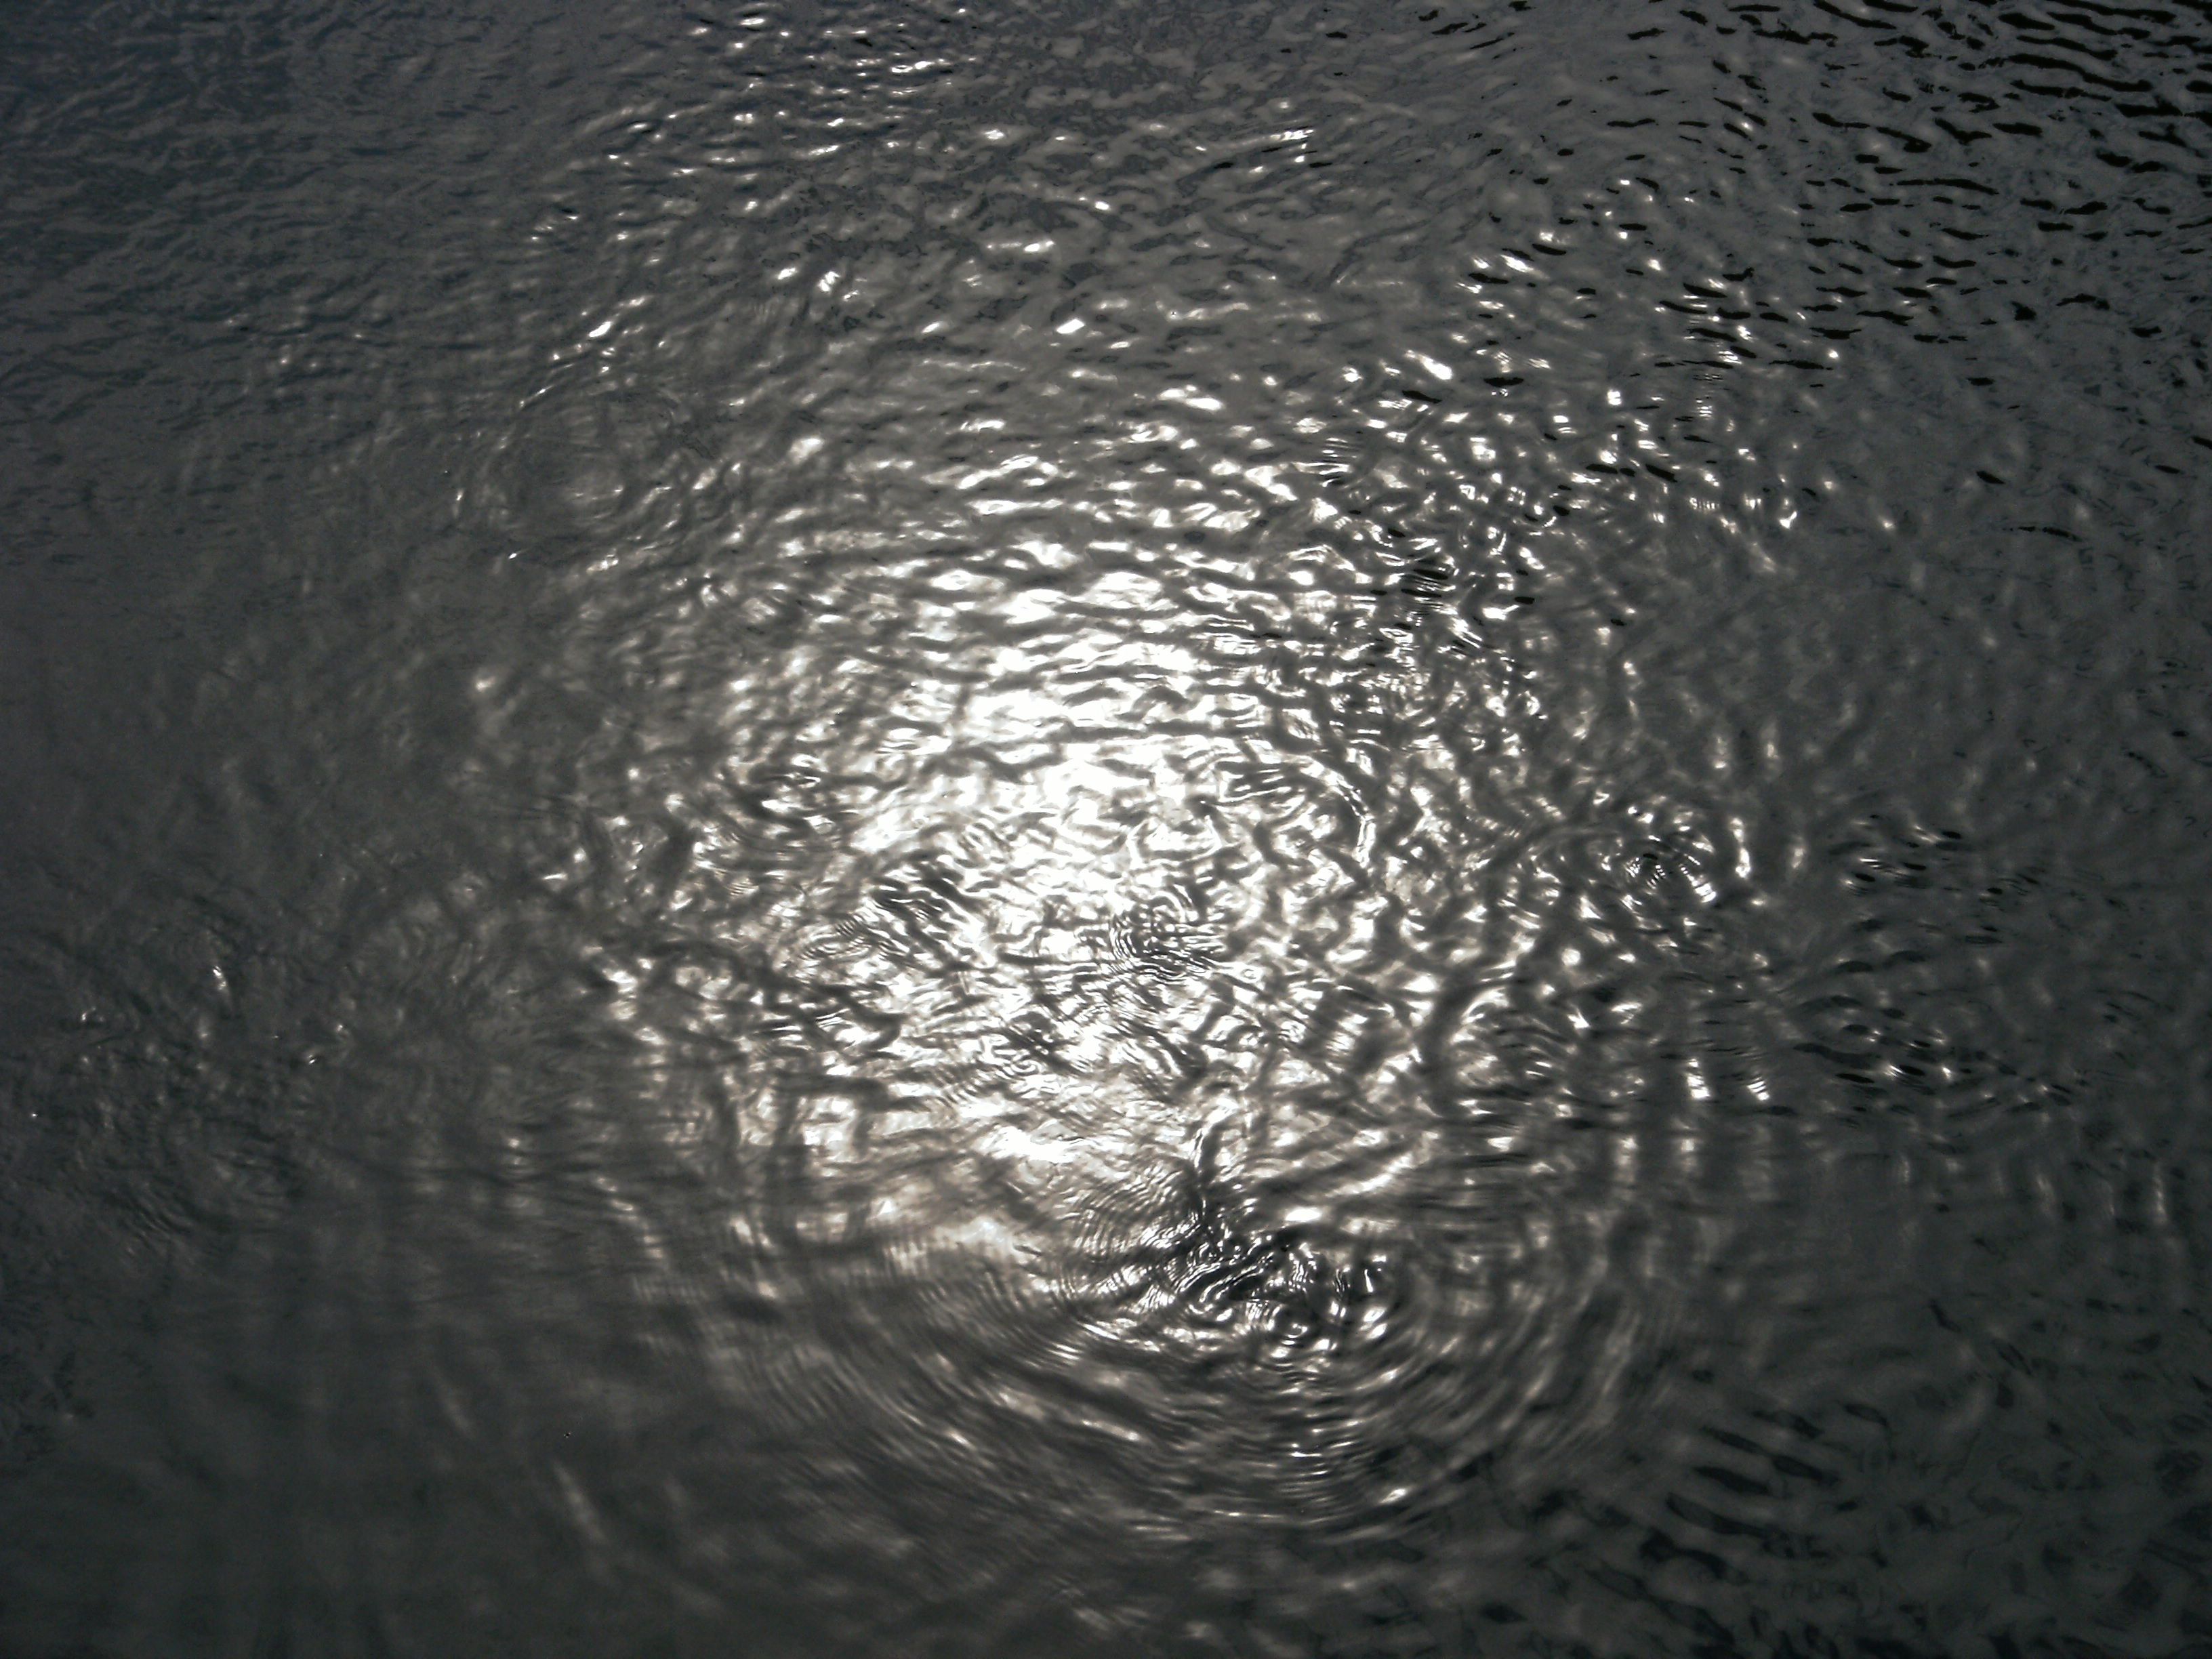
\includegraphics[width=.495\textwidth]{Images/Attribute/Sunglint_far_from_horizon}}
    \subcaptionbox{Source: Public domain. \label{fig:sunglintpyramid}}{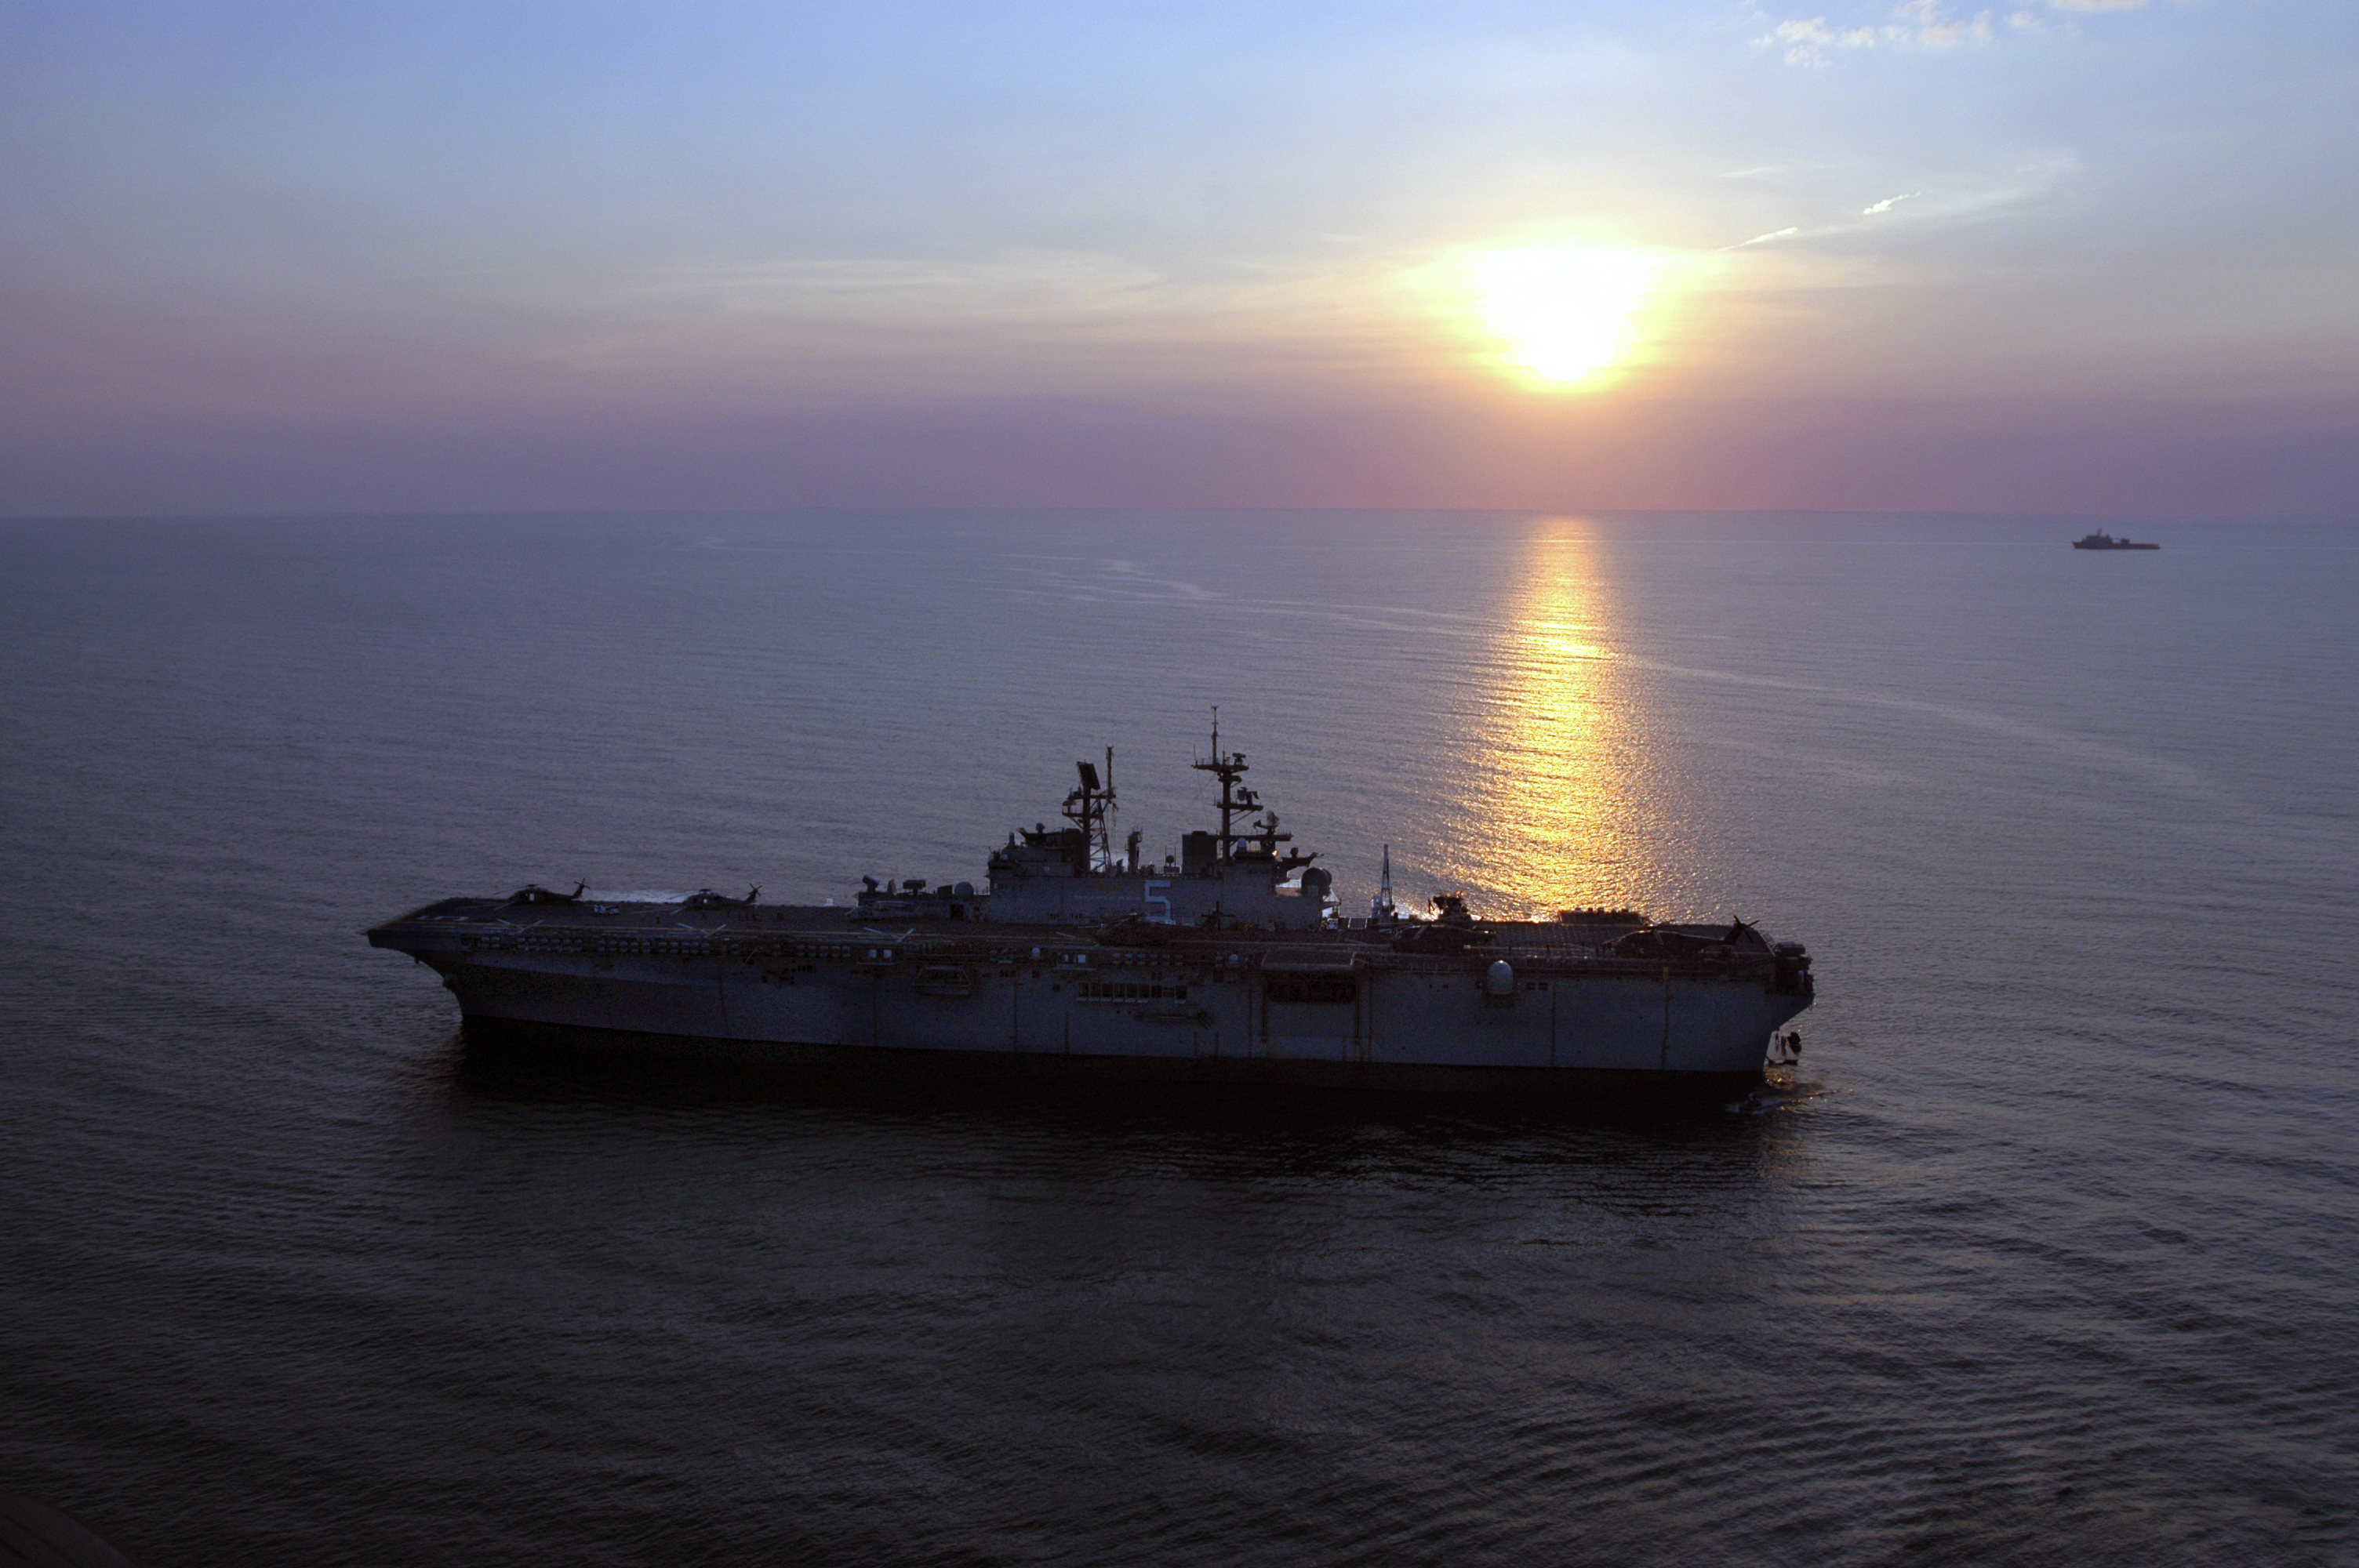
\includegraphics[width=0.495\textwidth]{Images/Public_domain/Sunglint_close_to_the_horizon}}
    \caption{When the surface is viewed from a close distance, the individual waves are clearly visible and there are clear borders between regions where the surface mirrors the sun, so called sun glitter, and regions where it does not. When the distance to the surface increases, the waves appear smaller and become hard to distinguish from one another, and the sun glitter is blended together with the regions that do not reflect the sun, giving rise to a diffuse reflection called sunglint. Both the shape of the sunglint seen in \subfigref{fig:sunglintegg} as well as the shape of the sunglint seen in \subfigref{fig:sunglintpyramid} can be explained by the model derived in this appendix.
    \subrefp{fig:sunglintegg} Sunglint shape caused by the sun being far from the horizon. The sunglint is slightly elliptical, or egg shaped, as long as the sun isn't at the zenith, for which it is circular. The more waves there are, the larger and the more egg shaped it will be. In this image it is still clear that the reflection of the sun is specular.
    \subrefp{fig:sunglintpyramid} Sunglint shape caused by the sun being close to the horizon. The sunglint is almost shaped like a pyramid, with the sun in the top vertex. The angle of the vertex depends on what the sea state looks like, the higher the waves, the wider the angle. In this image, the waves are too small to be clearly visible individually, and the reflection appears diffuse.
    }
    \label{fig:sunglints}
\end{figure}

One of the most well known and popular shading models in computer graphics is an adaption of the Phong shading model \citep{Phong1975} made by \citet{Blinn1977}, which is generally referred to as the \idxs{Blinn--Phong}{shading model}. While the Phong shading model works well for surfaces facing the viewer, and produces circular highlights, which are shaped similarly to the reflection that can be seen in \figref{fig:sunglintegg}, it doesn't perform well for surfaces viewed from a glancing angle, such as the one in \figref{fig:sunglintpyramid}. The adaption Blinn made changed the shape of the specular reflection from always being circular, to becoming more and more narrow as the angle the surfaces is viewed from decreases, which more closely resembles reality.

For water surfaces, this gives rise to a specular highlight that is elliptical, or slightly egg shaped, when the sun stands high in the sky, as can be seen in \figref{fig:sunglintegg}, and pyramid shaped when the sun is close to the horizon, with the sun in the top of the pyramid, as can be seen in \figref{fig:sunglintpyramid}.

By comparing the \idxs{shading}{model} derived in this appendix (\eqrefs \ref{eq:rendering_equation_simplified} and \ref{eq:spectral_radience_reflected_point_light_source}) to the Blinn--Phong shading model, it may be noticed that if the \idxs{wave}{spectra} $S$ is \idxse{circular}{symmetry}{circularly symmetric}, the factor $f(\nabla\eta^*(\vec{r}\,))$ (described by \eqref{eq:eta_grad_distribution_r_uniformly_distributed}) --- which is what gives the reflection of the point light source its shape --- becomes practically equivalent to the specular reflection term in the Blinn--Phong shading model except from a constant factor. This holds even though the Blinn--Phong shading model is based on experimental measurements of reflections from real surfaces and is developed mainly for solids, while the shading model presented in this appendix is specifically derived for water surfaces.

For symmetric wave spectra and for almost smooth surfaces (when the diffusion in the reflection of objects becomes very small), all factors in \eqref{eq:spectral_radience_reflected_point_light_source} except from $f(\nabla\eta^*(\vec{r}\,))$ vary very slowly in comparison to $f(\nabla\eta^*(\vec{r}\,))$ unless the surface is viewed from a glancing angle, and so the shape of the specular reflection can be \approximated as just a constant times $f(\nabla\eta^*(\vec{r}\,))$. Hence, the result of using \eqref{eq:spectral_radience_reflected_point_light_source} becomes very similar to the result of using the Blinn--Phong shading model, with the only practical difference that the reflection of a point light source according to the shading model derived in this appendix varies in intensity depending on how steep the angle is with which the observer sees the reflection, according to the factors $\anormvec{h}^4/(\normvec{\omega}_{\text{o}}\cdot\anormvec{n})$ and $R_{\normvec{n}^*\!,x}(\normvec{\omega}_{\text{o}})$; these are not included in the specular term in the Blinn--Phong shading model.

However, when the point light source is located low and the reflection comes relatively close to the horizon in comparison to the vertical spread of the reflection, the factor $\anormvec{h}^4/(\normvec{\omega}_{\text{o}}\cdot\anormvec{n})$ will vary more noticeably.

This becomes especially apparent when the reflection almost reaches the horizon, in which case real waves would start to mask each other out at the top of the diffuse reflection of the light source. If the surface is assumed to consist of V-groove cavities \citep{Torrance1967}, this masking occurs roughly above one third from the horizon to the center of the reflection. Since our model doesn't account for masking, the radiance directed against the observer will go to infinity when $\normvec{\omega}_{\text{o}}\cdot\anormvec{n}$ goes to 0, which is an unphysical behavior.

Furthermore, when the light source is very close to the horizon, real waves would start to shadow each other. By modeling the surface as V-groove cavities, this would start to occur roughly below a distance from the horizon that is three times the distance between the horizon and the light source, and the radiance directed against the observer would go to zero when the distance between the horizon and the light source went to zero. This is not the case in our model since it doesn't account for shadowing.

Masking and shadowing is generally referred to as geometric attenuation. \citet{Torrance1967} modeled the surface as a sequence of V-groove cavities, which allowed the attenuation to be modeled analytically. This V-groove cavity model has since been borrowed several times \citep{Blinn1977,Oren1994}, and could also be used to model geometric attenuation for the shading model derived in this appendix to prevent overly bright parts of the surface close to the horizon.

However, even this model is a too crude approximation in certain cases, for example when the surface is viewed from an extremely grazing angle, like the thin strip closest to the horizon. From this angle, almost every visible part of the surface is at the crest of a wave, since the rest of the wave is hidden behind other waves. Since the crest is on the top of a wave, naturally the surface gradient will be very low, which makes the surface more mirror-like, as can be seen in \figref{fig:sunglintpyramid}. This is not the case for the V-groove cavity model, where the entire cavity has the same slope.